\section{Data and Event Selection}\label{sec:ciEvSel}

The search for non-resonant features in the dilepton invariant-mass spectra is concerned with collisions that produce two leptons.
This section details the event selection, data, and simulation used in the analysis.
Finally, comparisons between the recorded data and simulation are provided.


\subsection{Event Selection}
During Run 2, roughly $10^{16}$ proton collisions took place in ATLAS. \check
Since many of these events are uninteresting for a dilepton analysis, only events meeting appropriate criteria are considered.
This reduces the total number of data events considered for the analysis to {\color{red}XXX} dimuon events and {\color{red}YYY} dielectron events.

% GRL
Only events recorded during good operation of the detector are used.
The events meeting this requirement comprise the Good Run List, summarized in Section \ref{sec:physData}.

% Trigger
The first requirement for an event to be considered is the trigger: events must be identified as interesting by the ATLAS trigger system in order to be recorded.
The triggers used during data collection differ from year to year. 
In the dielectron channel, the following trigger requirements are applied.
\begin{itemize}
	\item 2015: 2e12\_lhloose\_L12EM10VH
	\item 2016: 2e17\_lhvloose\_nod0
	\item 2017 and 2018: 2e24\_lhvloose\_nod0
\end{itemize}
Although events passing these triggers are expected to contain two electrons, both may not be reconstructed. 
A subsequent requirement for two electrons to be reconstruction is made in the following selection.

In the dimuon channel, the following trigger requirements are applied.
\begin{itemize}
	\item 2015: mu26\_imedium or mu50
	\item 2016, 2017 and 2018: mu26\_ivarmedium or mu50
\end{itemize}
These trigger on events with single isolated muons. 
The choice to use these, rather than a two muon trigger, was made to increase the trigger's efficiency for dimuon events.
The requirement for an event to have two muons is made in the following selection.

% Object selection
After passing the trigger requirement, events are evaluated under selection criteria.
In events where multiple vertices are reconstructed, the vertex with the largest $\sum\pt^2$ is the \emph{primary vertex}.
Events are required to have two Inner Detector tracks associated with the primary vertex.
The first step is to define what objects are considered in each event, based on the object definitions from Section \ref{sec:physObjects}.
Many of the technical terms used here follow the definitions found in that section.

Next, specific requirements are made as to where the objects were reconstructed in the detector. 
This defines the fiducial region in which the search is carried out.
This definition differs for electrons and muons.

Electrons are defined using the \code{MediumLLH} identification.
They are required to pass \emph{Gradient} isolation.
Additionally, they must not be from a ``bad'' calorimeter cluster (\code{BADCLUSELECTRON}), and several other requirements.
The electron energy is calibrated using \code{es2017\_R21\_v1} (\code{ESModel}).
An additional loose selection for electrons is also made, called the \emph{loose selection}, to study electron systematics.
This is otherwise the same as the nominal electron selection.
The kinematic criteria for both electron selections are listed in Table \ref{tab:ciElectronSel}.

\begin{table}[!htb]
\caption{Selection criteria for electrons. Parameters $d_{0}$ and $z_{0}$ are the transverse and longitudinal displacements of the track associated with the electron, and the vertex.}
\begin{center}
    \begin{tabular}[ht]{l l}
    \toprule
    Feature & Criteria \\
    \midrule
    Pseudorapidity range & $(|\eta| < 1.37) \quad || \quad (1.52 < |\eta| < 2.47)$ \\
    Transverse momentum & p$_T$ $>$ 30~GeV \\
    Track impact parameter significance & $|d_{0}^{BL}(\sigma)|$ $<$ 5 \\
    Track $z$ displacement & $|\Delta z_{0}^{BL} \sin{\theta}| <$ 0.5~mm \\
    \bottomrule
    \end{tabular}
\end{center}
\label{tab:ciElectronSel}
\end{table}

Muons are defined using the High-$p_T$ selection working point and must pass the \code{FCTightTrackOnly} isolation requirement.
An additional cut, the \emph{Bad Muon Veto}, is required to reject muons with large \pt uncertainty.
The remaining kinematic criteria for muons are given in Table \ref{tab:ciMuonsSel}.

\begin{table}[ht]
\caption{Selection criteria for muons. Parameters $d_{0}$ and $z_{0}$ are the transverse and longitudinal displacements of the track associated with the muon, and the vertex.}
\begin{center}
    \begin{tabular}[ht]{l l}
    \toprule
    Feature & Criteria \\
    \midrule
    Transverse momentum  & $\pt>30$ GeV\\
    Pseudorapidity range & $|\eta|<2.5$ \\
    Track impact parameter significance & $|d_{0}^{BL}(\sigma)|< 3$ \\
    Track $z$ displacement  & $|\Delta z_{0}^{BL} \sin{\theta}| < 0.5~mm$\\
    \bottomrule
    \end{tabular}
\end{center}
\label{tab:ciMuonsSel}
\end{table}

Occasionally, the interaction of a single particle with detectors results in the reconstruction of two particles.
To avoid this, and \emph{overlap removal} scheme removes particles that are suspiciously close to each other.
The criteria are listed in Table \ref{tab:ciOr}.
\begin{table}[ht]
\caption{Overlap removal}
\begin{center}
    \begin{tabular}[ht]{l l l}
    \toprule
    Reject & Against & Criteria \\
    \midrule
    Electron & Electron & Shared ID track, $\pt^1<\pt^2$ \\
    Muon     & Electron & Is calo-muon and shared ID track \\
    Electron & Muon     & Shared ID track \\
    \bottomrule
    \end{tabular}
\end{center}
\label{tab:ciOr}
\end{table}
Further rejection of muons and electrons takes place if a jet is reconstructed within an angular distance $\delta R<0.4$.

% Event selection
The requirements listed so far define a set of events to consider, and a set of objects in each event.
It remains to determine whether the event is interesting with respect to the present analysis.
In general, events containing either two electrons or two muons are of interest.
Of the same-flavor leptons in the event, the leading and subleading \et (\pt) pair are selected in the electron (muon) channel.
In the muon channel, only pairs of oppositely charged muons are considered. 
In the electron channel, the charge is ignored since bremsstrahlung emission of photons can lead the electron track to bend, leading to the miss-identification of the charge.
Finally, a preliminary invariant mass cut of $\mll>130$~GeV is required.
In the case where both a dielectron and dimuon candidate meet these requirements, the dielectron is selected, and the dimuon is discarded.
This choice is made due to the preferable electron \et resolution at high energy.

\subsection{Data}
The data used in this analysis were collected during the LHC's Run 2.
The recorded integrated luminosity of the collisions is $139\pm2$ \fb. \cite{ATLAS-CONF-2019-021}

The data yield rate, broken into the different runs and periods for each year, are shown in Figure ~\ref{fig:ciYields}.
These plots count events after applying the full selections.

\begin{figure}[ht!]
\captionsetup[subfigure]{position=b}
\centering
\subfloat[][]{{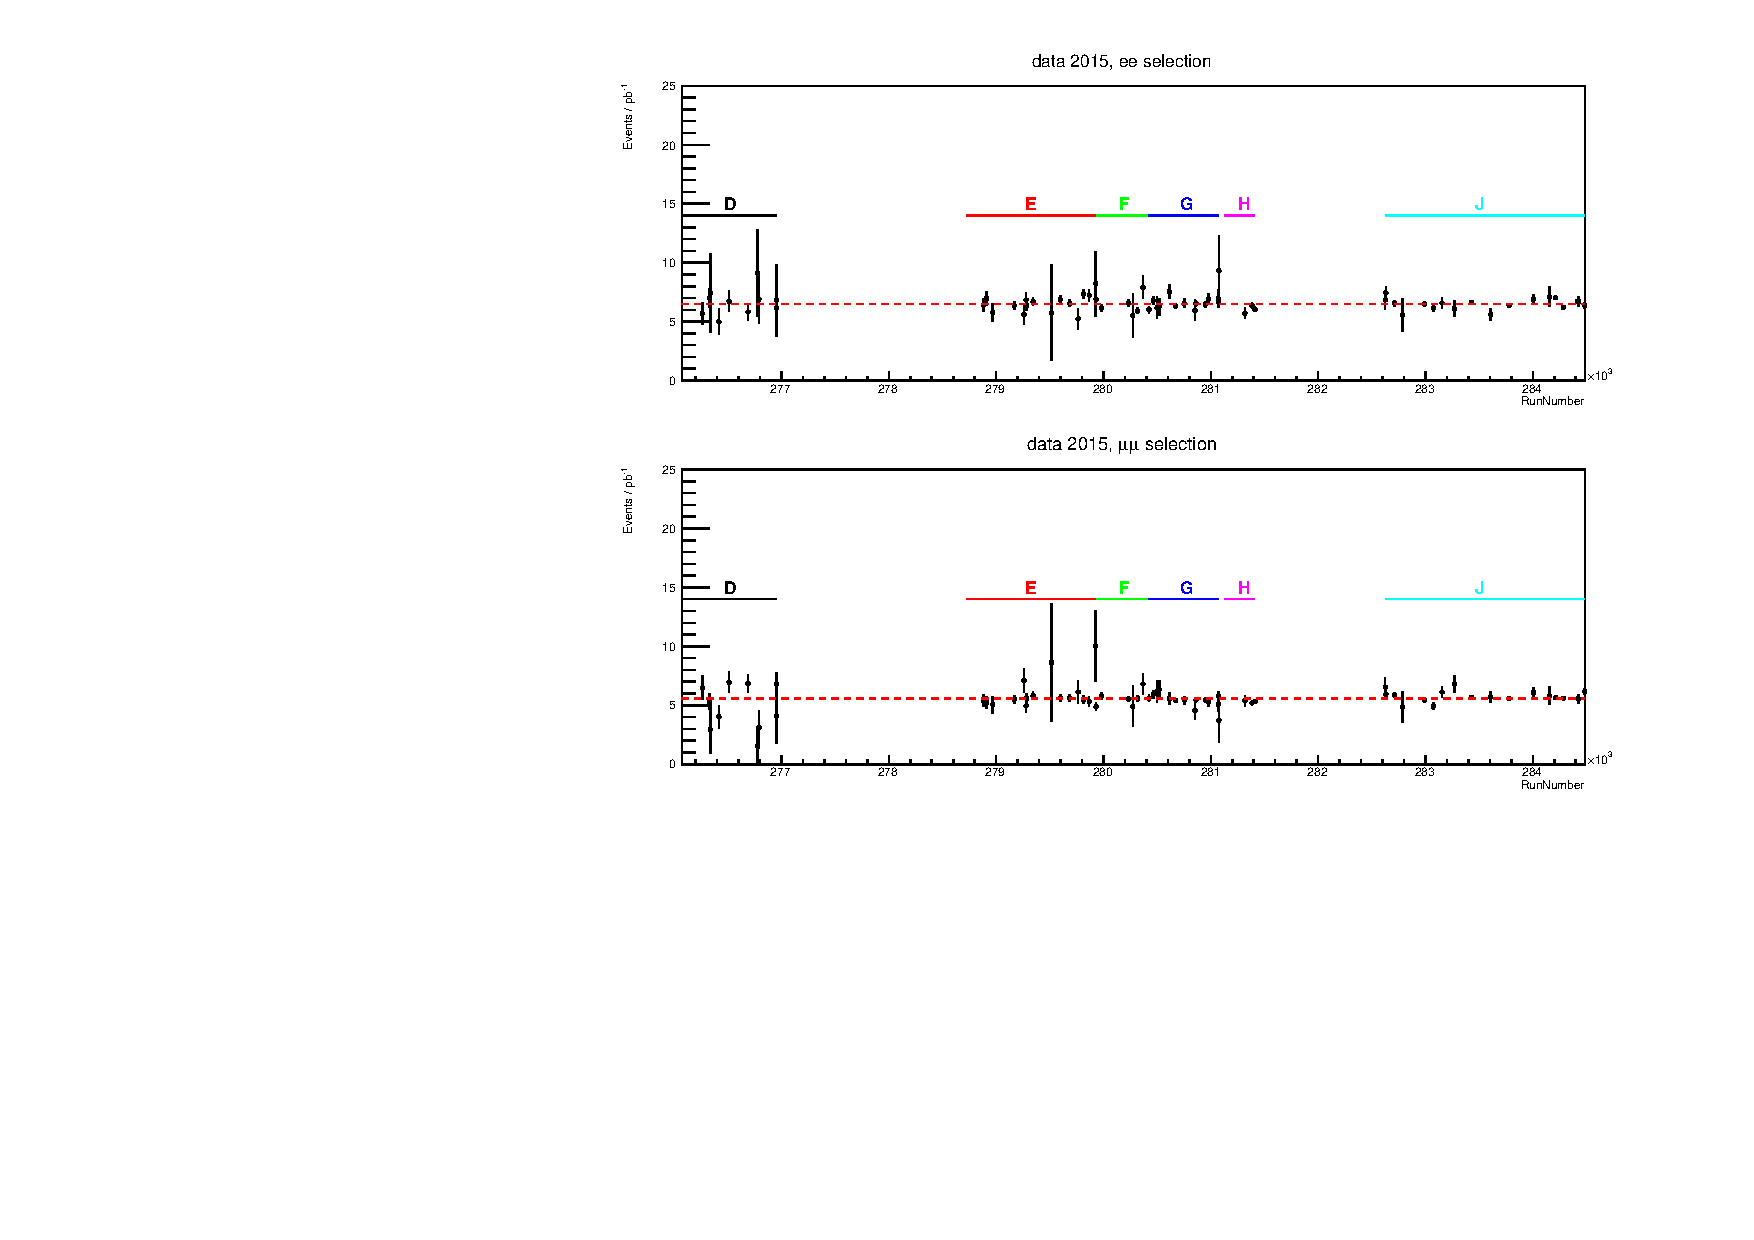
\includegraphics[width=0.48\textwidth]{figures/ci/dataMc/compare_data_yields2015.pdf}}}
\subfloat[][]{{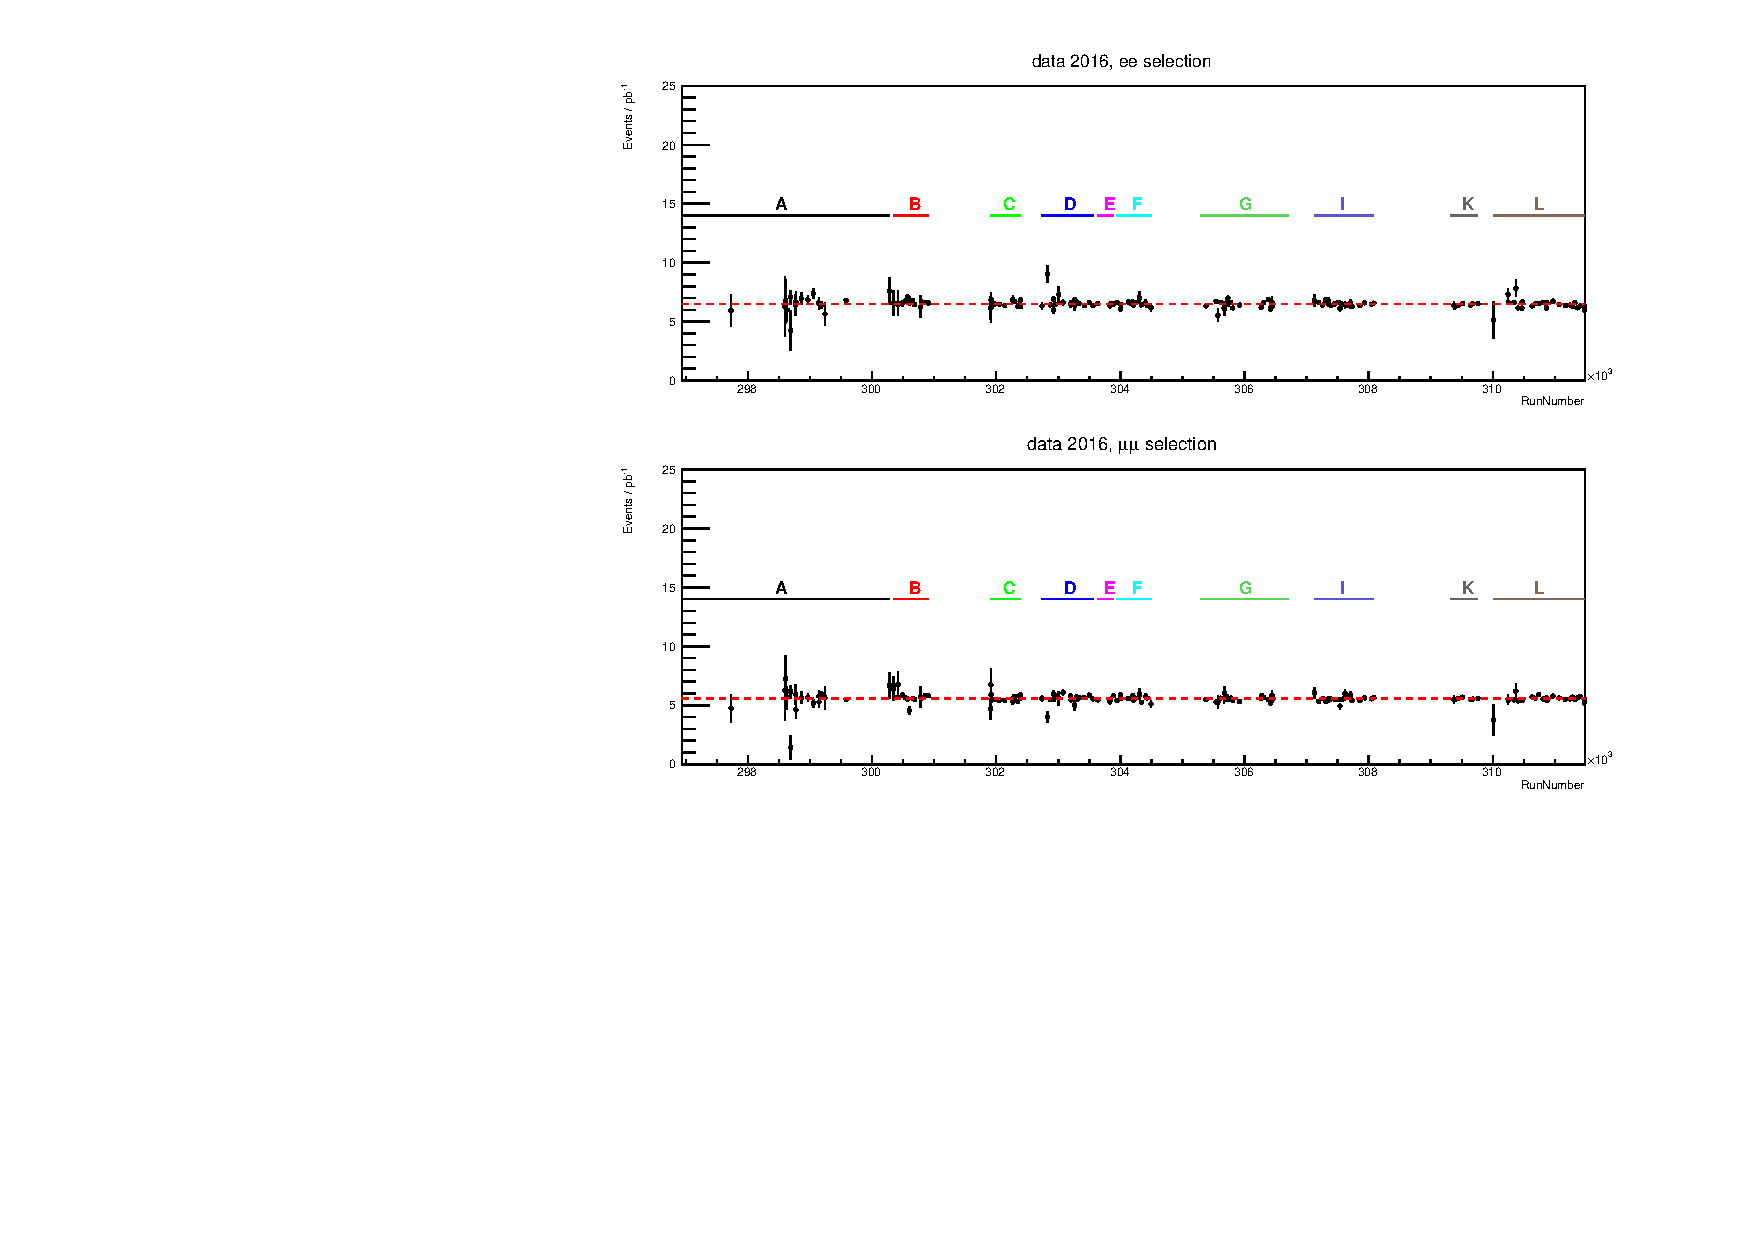
\includegraphics[width=0.48\textwidth]{figures/ci/dataMc/compare_data_yields2016.pdf}}}\\
\subfloat[][]{{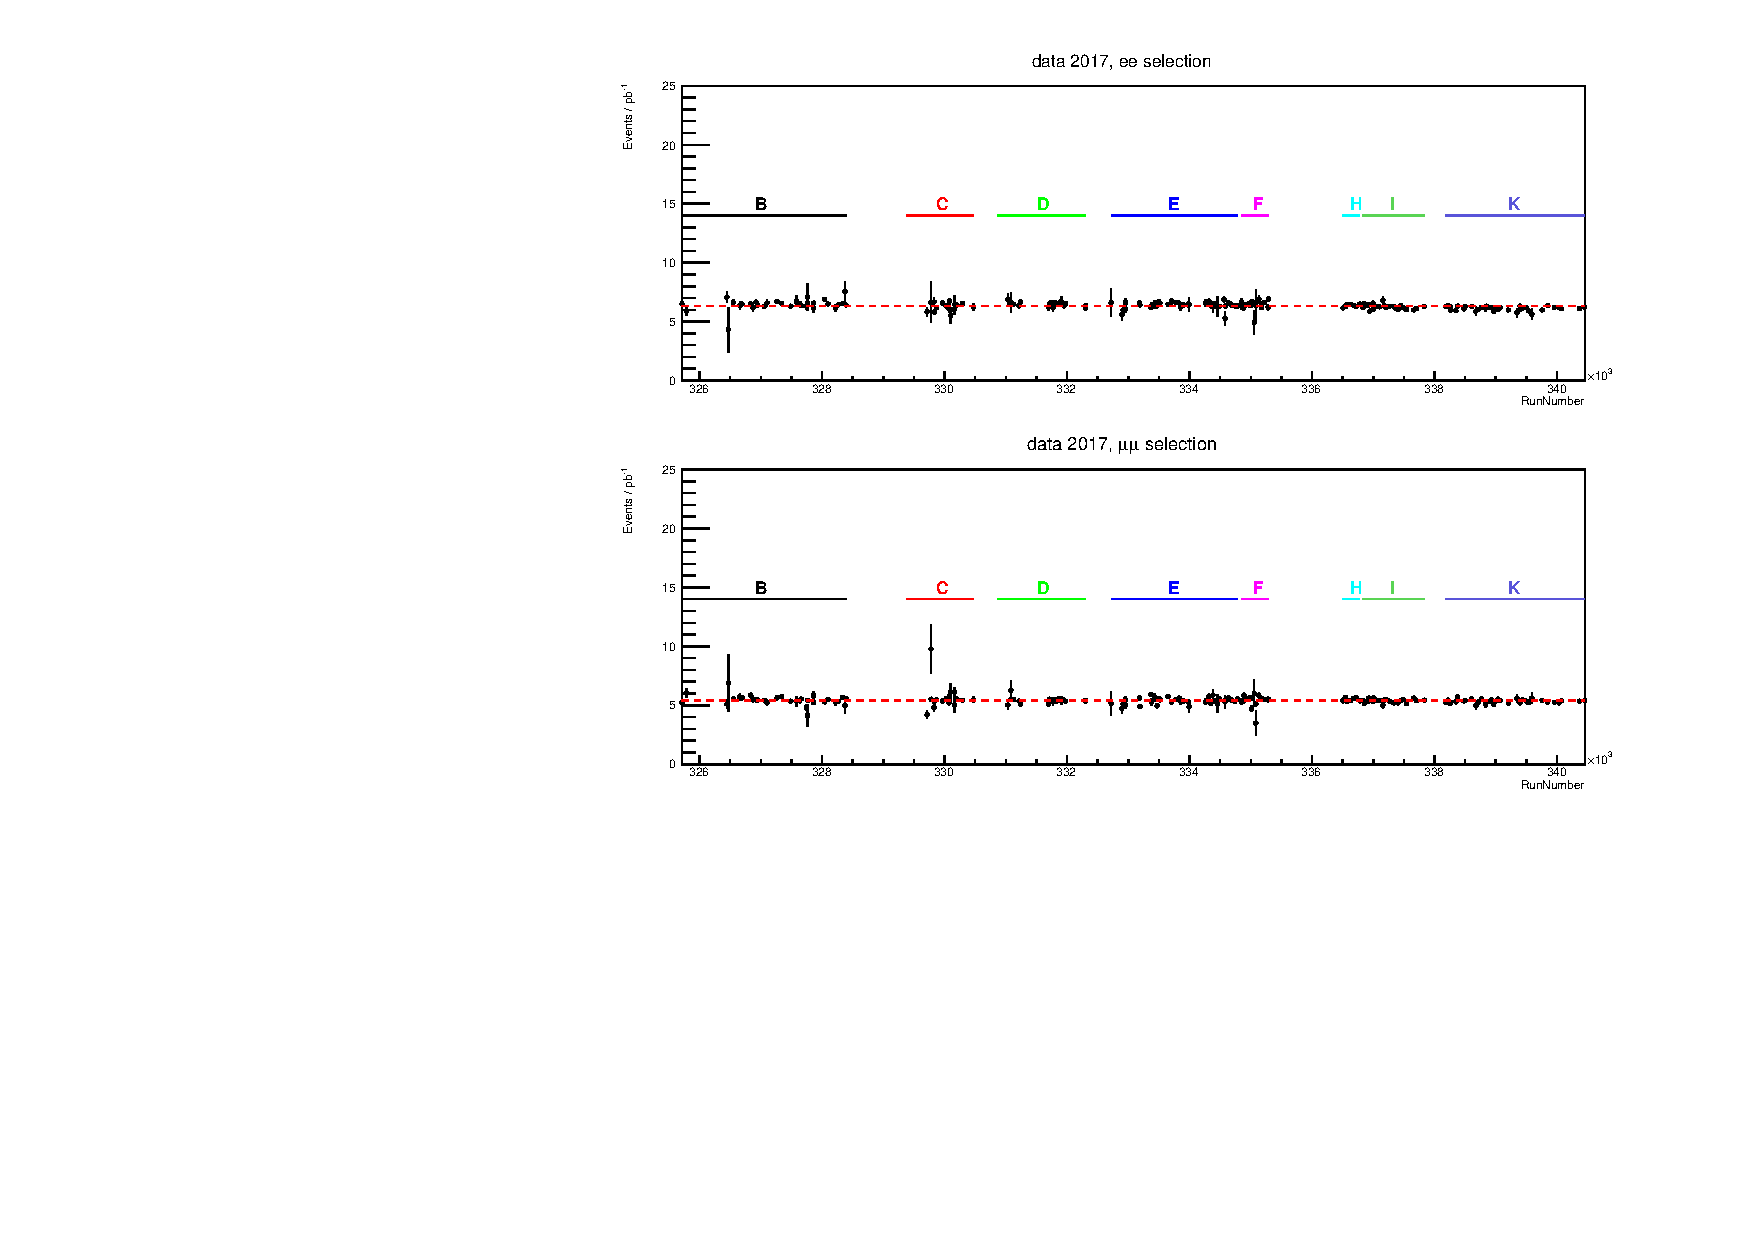
\includegraphics[width=0.48\textwidth]{figures/ci/dataMc/compare_data_yields2017.pdf}}}
\subfloat[][]{{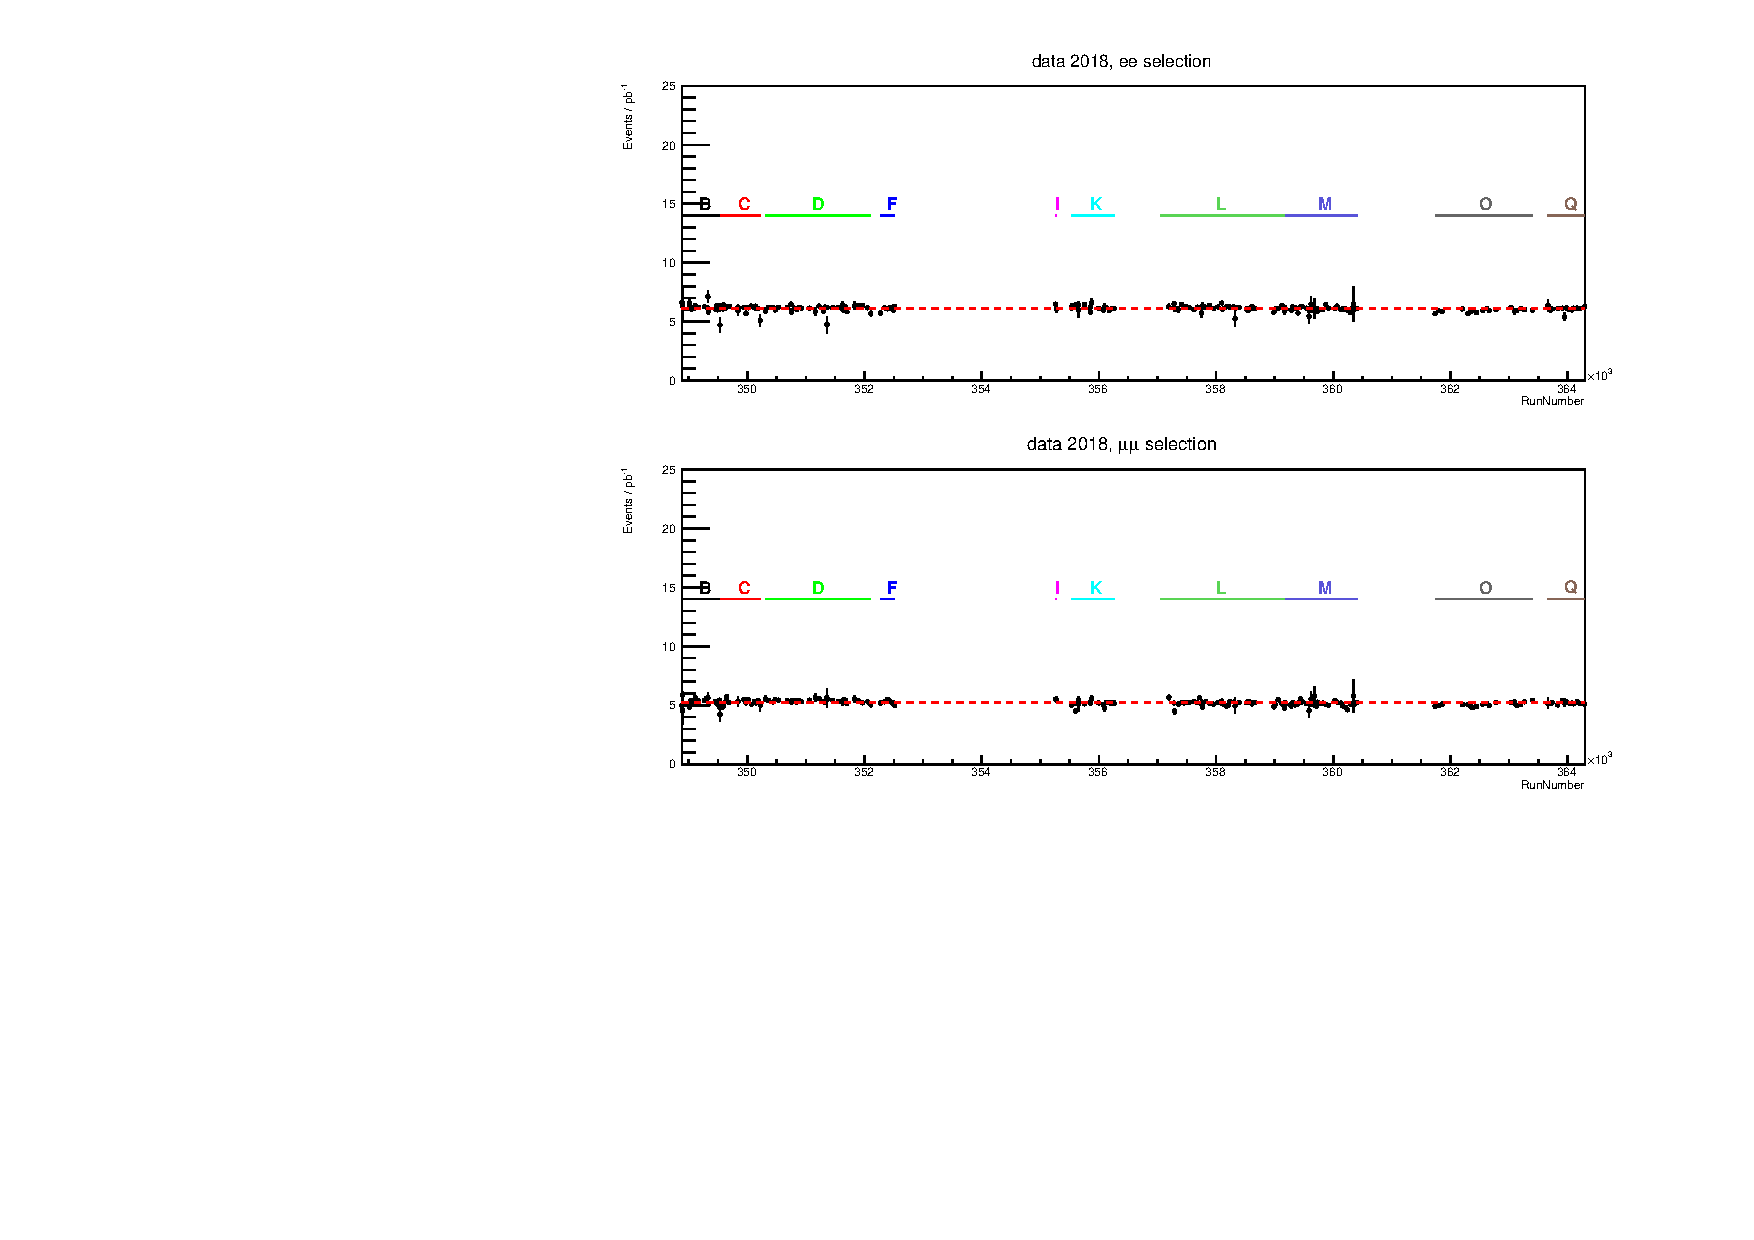
\includegraphics[width=0.48\textwidth]{figures/ci/dataMc/compare_data_yields2018.pdf}}}
\caption{Data yields for the each run period for the inclusive $ee$ (above) and $\mu\mu$ (below) selections.}
\label{fig:ciYields}
\end{figure}
\clearpage

\subsection{Simulation}

This analysis uses simulated invariant-mass distributions for three purposes:
\begin{enumerate}
    \item Modeling the CI signal. This is done using simulated DY events, reweighted to include interference and direct production from a contact interaction.
    \item Testing a variety of choices made during the analysis. In particular, with respect to choosing a functional form that matches the expected background shape and with respect to choosing the control and signal regions.
    \item Measuring the impact of experimental and theoretical uncertainties on the results.
\end{enumerate}

All simulation-based background contributions are scaled by their respective cross-sections and summed to obtain the simulated background $m_{\ell\ell}$ distribution.
The main simulated backgrounds in decreasing order of contribution to the full mass spectrum are Drell--Yan (DY), top-quark pair ($t\bar{t}$), single-top-quark, and diboson production.
The multi-jet and $W+$jets processes in the dielectron channel are estimated from the data using the matrix method similar to Ref.~\cite{EXOT-2016-05}. The contribution of such processes to the analysis is estimated using a likelihood fit.
The same processes in the dimuon channel, as well as processes with $\tau$-leptons in both channels, have a negligible impact and are not considered.
The Monte Carlo (MC) event generators for the hard-scattering process and the programs used for parton showering are listed in Table~\ref{tab:MC} with their respective parton distribution functions (PDFs).
Afterburner generators such as \textsc{Photos}~\cite{Golonka:2005pn} for the final-state photon radiation (FSR) modeling, \textsc{MadSpin}~\cite{Artoisenet:2012st} to preserve top-quark spin correlations, and \textsc{EvtGen}~\cite{Lange:2001uf} for the modeling of $c$- and $b$-hadron decays, are also included in the simulation.

\begin{table}[htbp]
\centering
\caption{The programs and PDFs used to generate the hard-scatter matrix element (ME) and to simulate parton showering (PS) in the signal and background processes.
The top-quark mass is set to 172.5 GeV.}
{\scriptsize
\begin{tabular}{lll}
\toprule
Background Process & ME Generator and ME PDFs & PS and non-perturbative effect with PDFs \\\hline
NLO Drell--Yan & \POWHEGBOX~\cite{Alioli:2010xd,Frixione:2007vw}, CT10~\cite{ct10}, \textsc{Photos} & \PYTHIAV{v8.186}~\cite{pythia8}, CTEQ6L1~\cite{ATL-PHYS-PUB-2014-021,Stump:2003yu}, \textsc{EvtGen1.2.0} \\
$t\bar{t}$  & \POWHEGBOX, NNPDF3.0NLO~\cite{Ball:2014uwa} & \PYTHIAV{v8.230}, NNPDF23LO~\cite{Ball:2012cx}, \textsc{EvtGen1.6.0} \\
Single top $s$-channel, $Wt$& \POWHEGBOX, NNPDF3.0NLO & \PYTHIAV{v8.230}, NNPDF23LO, \textsc{EvtGen1.6.0} \\
Single top $t$-channel & \POWHEGBOX, NNPDF3.04fNLO, \textsc{MadSpin} & \PYTHIAV{v8.230}, NNPDF23LO, \textsc{EvtGen1.6.0}  \\
Diboson ($WW$, $WZ$ and $ZZ$) & \SHERPA 2.1.1~\cite{Gleisberg:2008ta}, CT10 &\SHERPA 2.1.1, CT10  \\\hline
Signal Process & & \\\hline
LO Drell--Yan & \PYTHIAV{v8.186}, NNPDF23LO  &  \PYTHIAV{v8.186}, NNPDF23LO, \textsc{EvtGen1.2.0} \\
LO CI & \PYTHIAV{v8.186}, NNPDF23LO  &  \PYTHIAV{v8.186}, NNPDF23LO, \textsc{EvtGen1.2.0} \\
\bottomrule
\end{tabular}
}
\normalsize
\label{tab:MC}
\end{table}
SOFT-2010-01



The DY~\cite{ATL-PHYS-PUB-2016-003} and diboson~\cite{ATL-PHYS-PUB-2016-002} samples were generated in slices of dilepton mass to increase the sample statistics in the high-mass region.
Next-to-next-to-leading-order (NNLO) corrections in quantum chromodynamic (QCD) theory, and next-to-leading-order (NLO) corrections in electroweak (EW) theory, were calculated and applied to the DY events.
The corrections were computed with {\textsc{VRAP}} v0.9~\cite{vrap} and the CT14 NNLO PDF set~\cite{CT14} in the case of QCD effects, whereas they were computed with {\textsc{MCSANC}}~\cite{MCSANC} in the case of quantum electrodynamic effects due to initial-state radiation, interference between initial- and final-state radiation, and Sudakov logarithm single-loop corrections.
These are calculated as mass-dependent K-factors, and reweight simulated events before reconstruction.
The top-quark samples~\cite{ATL-PHYS-PUB-2016-020} are normalized to the cross-sections calculated at NNLO in QCD, including resummation of the next-to-next-to-leading logarithmic soft gluon terms as provided by \textsc{Top++}2.0~\cite{Czakon:2011xx}.

% Scale factors
The simulated data is weighted by several \emph{scale factors}, such that it more accurately represents reality.
These are listed here:
\begin{itemize}
	\item Pile-up reweighting weights.
	\item Mass dependant $K$-factors account for differences in the total cross-section if higher-order calculations are available for a given process compared to the order available in the MC samples. In the case of the LO and NLO DY samples, the SFs provide corrections for higher-order QCD, EW, and photon-induced (PI) effects.
	\item Experimental scale factors for leptons:
	\begin{itemize}
		\item Electrons: Reconstruction, trigger, isolation, and identification scales factors are applied.
		\item Muons: Reconstruction, trigger, isolation, and TTVA scale factors are applied.
	\end{itemize}
	\item Trigger scale factors according to the specific channel.
\end{itemize}

All fully simulated event samples include the effect of multiple $pp$ interactions in the same or neighboring bunch crossings.
These effects are collectively referred to as pile-up.
The simulation of pile-up collisions was performed with \PYTHIAV{v8.186} using the ATLAS A3 set of tuned parameters~\cite{ATL-PHYS-PUB-2016-017} and the NNPDF23LO PDF set, and weighted to reproduce the average number of pile-up interactions per bunch crossing observed in data.
The generated events were passed through a full detector simulation~\cite{SOFT-2010-01} based on\ \GEANT~4~\cite{geant}.

To reduce statistical uncertainties, a large additional DY sample is used where the detector response is modeled by smearing the dilepton invariant-mass with mass-dependent acceptance and efficiency corrections, instead of using the CPU-intensive \GEANT~4 simulation.
The relative dilepton mass resolution used in the smearing procedure is defined as $(m_{\ell\ell}-m_{\ell\ell}^\mathrm{true})/m_{\ell\ell}^\mathrm{true}$, where $m_{\ell\ell}^\mathrm{true}$ is the generated dilepton mass at Born level before FSR.
The mass resolution is parameterized as a sum of a Gaussian distribution, which describes the detector response, and a Crystal Ball function composed of a secondary Gaussian distribution with a power-law low-mass tail,
which accounts for bremsstrahlung effects or for the effect of low resolution in the muon momentum at high \pt.
The parameterization of the relative dilepton mass resolution as a function of $m_{\ell\ell}^\mathrm{true}$ is determined by a fit of the function described above to simulated DY events at NLO.
A similar procedure is used to produce a mass-smeared $t\bar{t}$ sample.
These two samples replace the equivalent ones produced with the full detector simulation wherever applicable in the remainder of the analysis.
The number of events in these samples is more than 55 times the number of events in data.
These samples would have been challenging to produce with the full detector simulation because of the large number of events required and the limited computing resources.

Signal $m_{\ell\ell}$ distribution shapes are obtained by a matrix-element reweighting~\cite{EXOT-2016-05} of the leading-order (LO) DY samples generated in slices of dilepton mass.
This reweighting includes the full interference between the non-resonant signal and the background DY process.
The weight function is the ratio of the analytical matrix-elements of the full CI (including the DY component) and the DY process only, both at LO.
It takes as an input the generated dilepton mass at Born level before FSR, the incoming quarks' flavor, and the CI model parameters ($\Lambda$, chirality states, and the interference structure).
These weights are applied to the LO DY events to transform these into the CI signal shapes, in steps of $2$~TeV between $\Lambda=12$~TeV and $\Lambda=100$~TeV.
Dilepton mass-dependent higher-order QCD production corrections for the signals are computed with the same methodology as for the DY background, correcting from LO to NNLO.
Similarly, electroweak corrections for the signals are applied in the CI reweighting along with the interference effects, correcting from LO to NLO.
These signal shapes are used for optimizations as well as for calculations of the cross-section and acceptance times efficiency.

\subsection{Kinematic Distributions}

Several distributions of kinematic variables are provided in the following figures.
First, the invariant mass distributions are shown in Figure \ref{fig:ciMassMcPlot}.
These plots show the distribution of simulated events along with data events for both \ee and \mm selections.
Several representative contact interaction shapes are included for reference.
These plots clearly show the relative composition of the background in the simulated distributions.
The plots of the \ee selection additionally include the multi-jet and $W+$jets background.
The following figures show some kinematic variables for each selection.
Fully simulated resonant signals are included in these as illustrations, as the CI signal is reweighted only in the invariant-mass distribution.

\afterpage{
\begin{figure}[h!]
\captionsetup[subfigure]{position=b}
\centering
 \begin{minipage}[b]{.45\linewidth}
    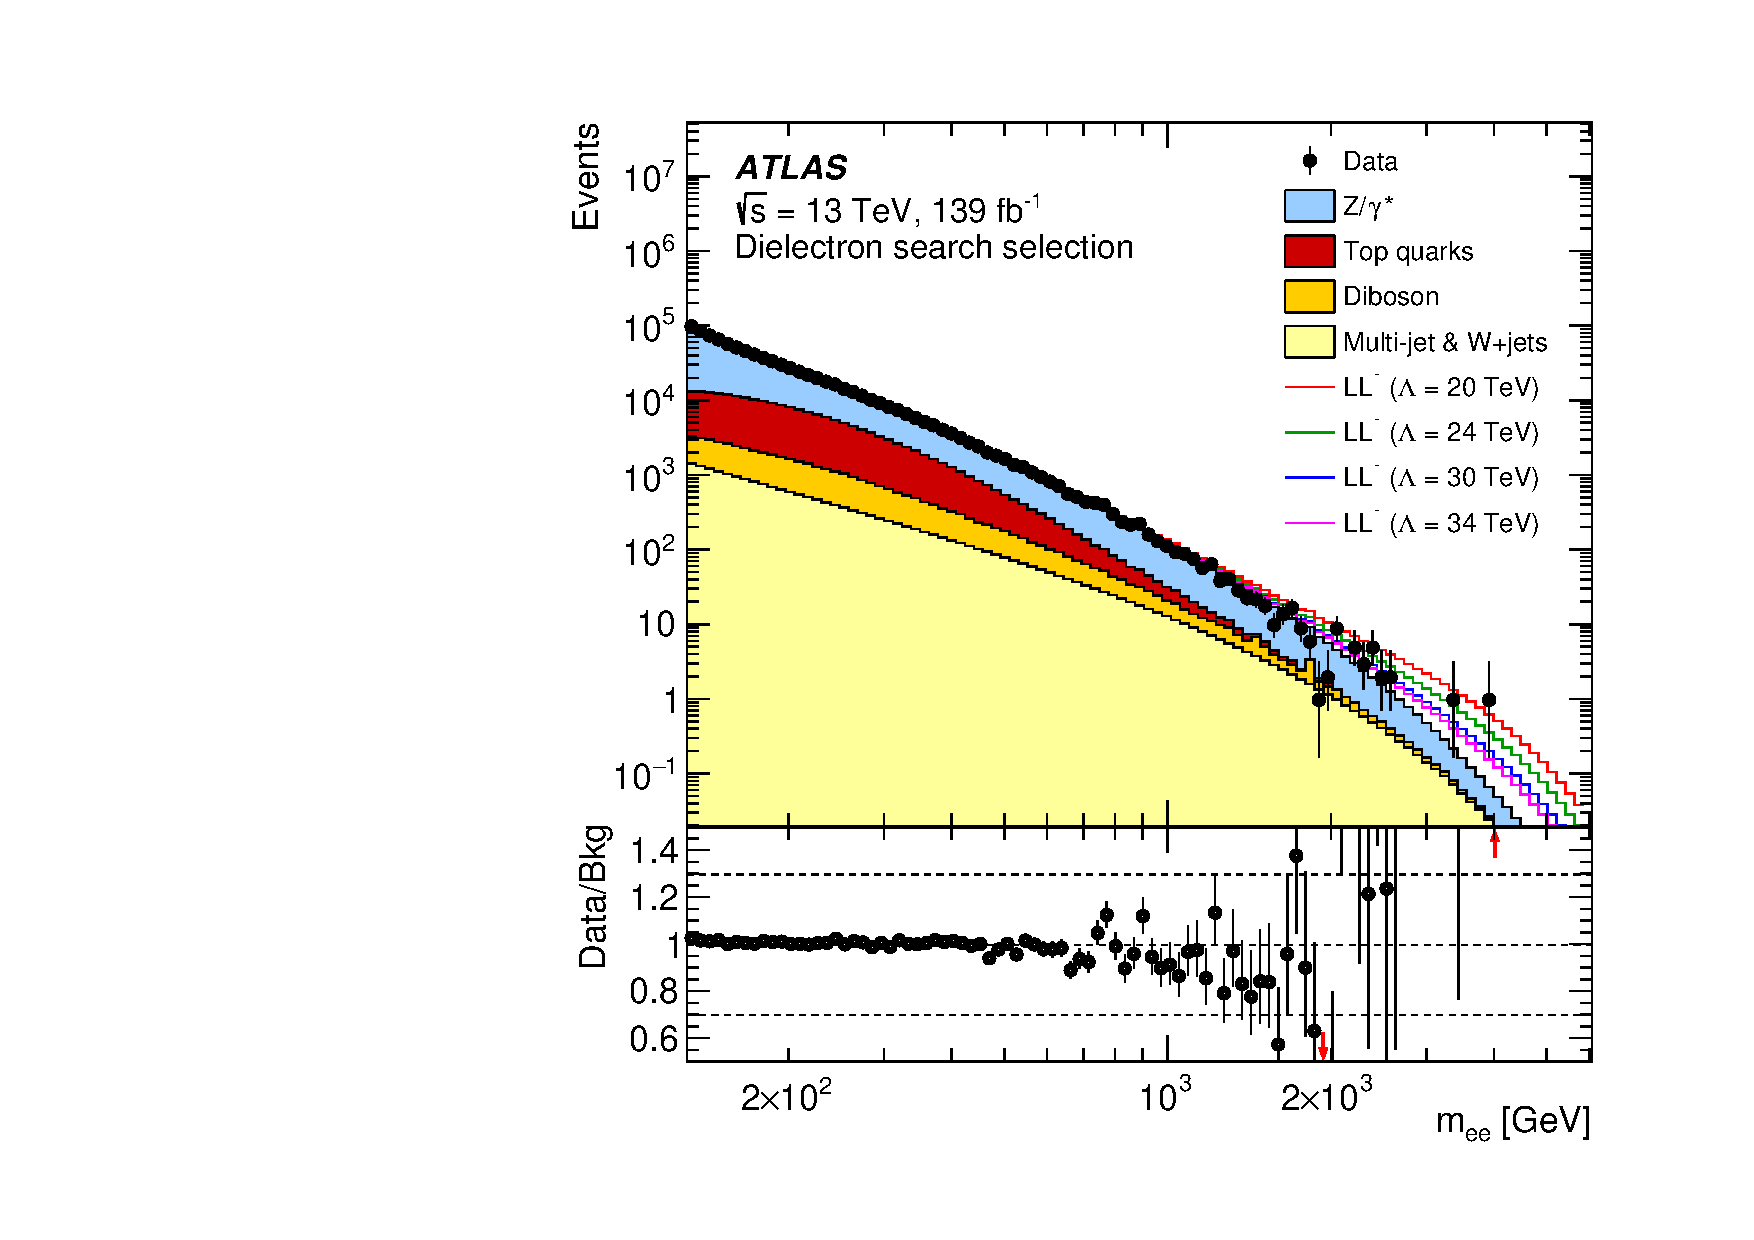
\includegraphics[width=1\textwidth]{figures/ci/dataMc/figaux_05a.pdf}
    \subcaption{}\label{fig:1a}
\end{minipage}
\begin{minipage}[b]{.45\linewidth}
    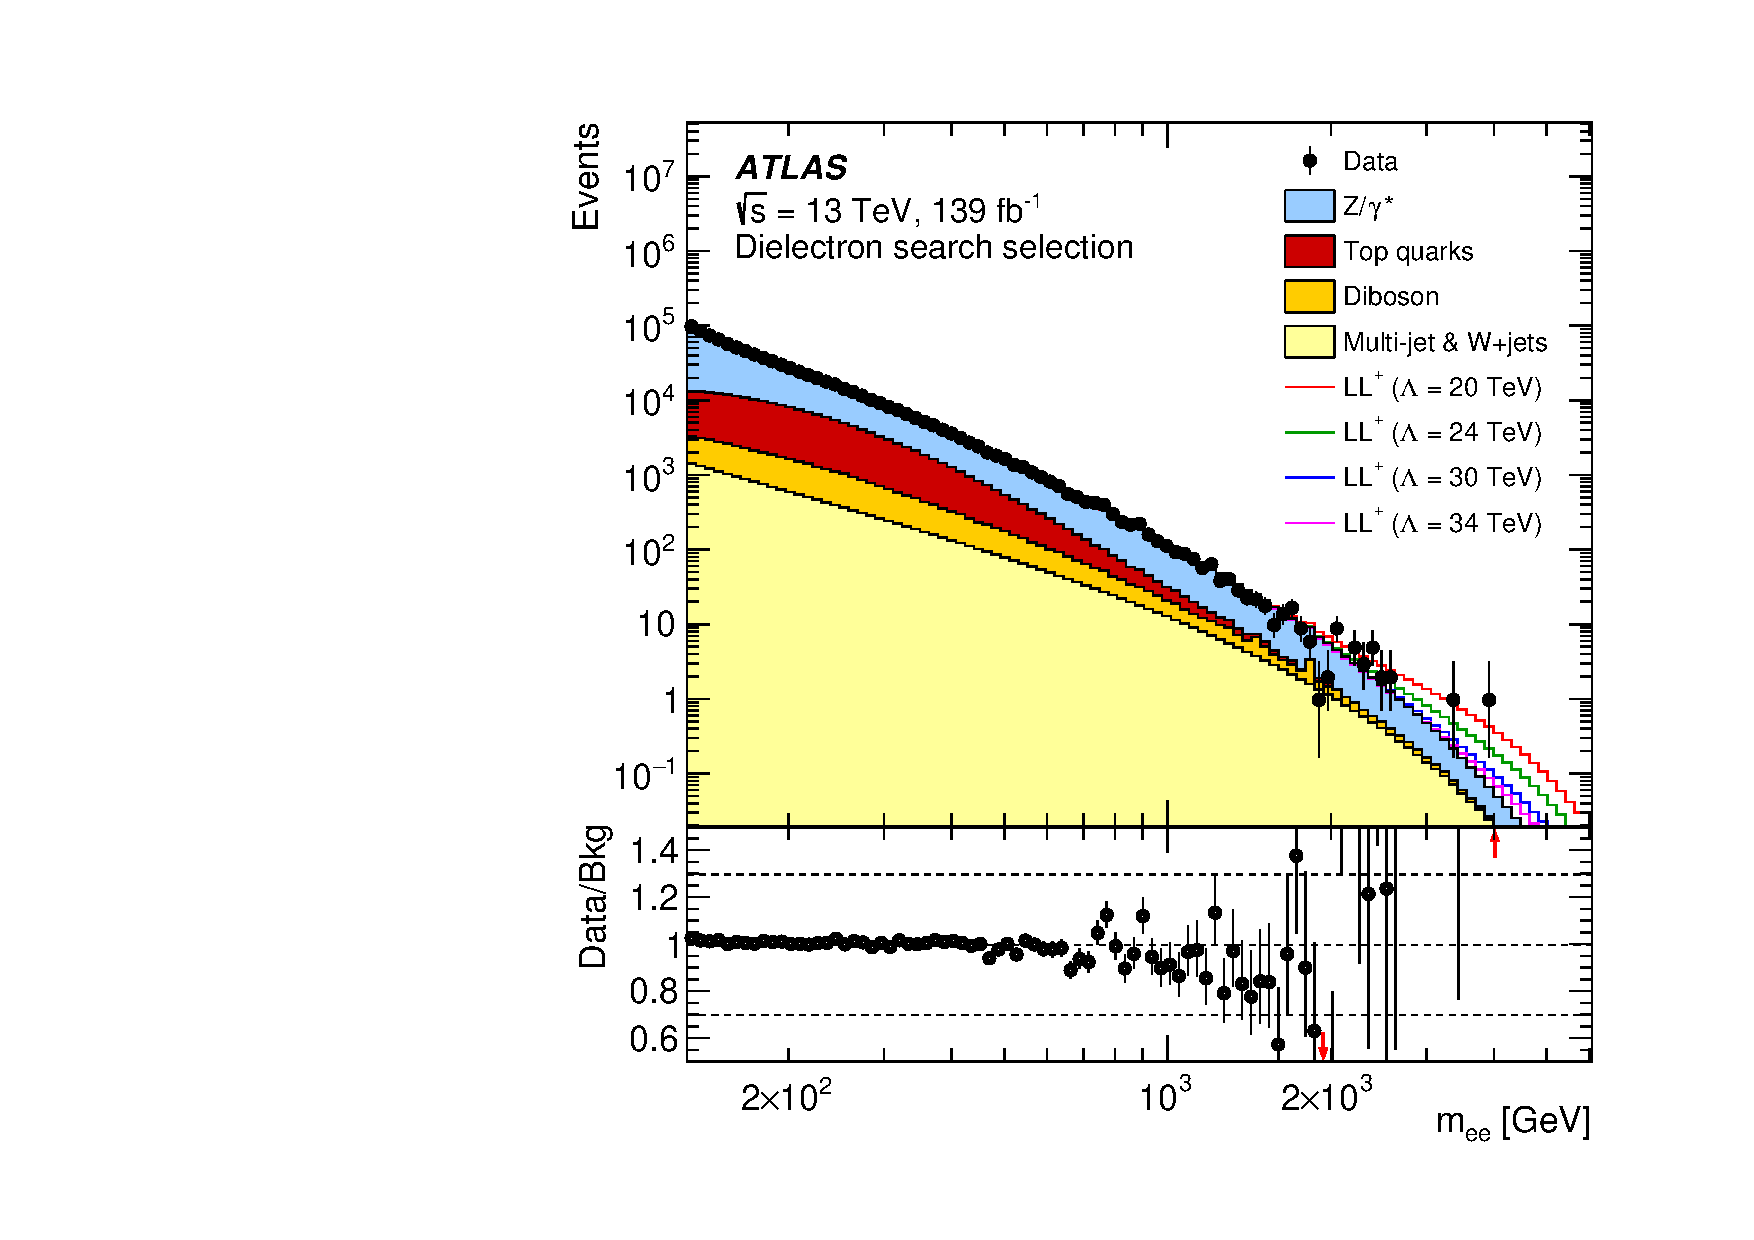
\includegraphics[width=1\textwidth]{figures/ci/dataMc/figaux_05b.pdf}
    \subcaption{}
\end{minipage} \\
\begin{minipage}[b]{.45\linewidth}
    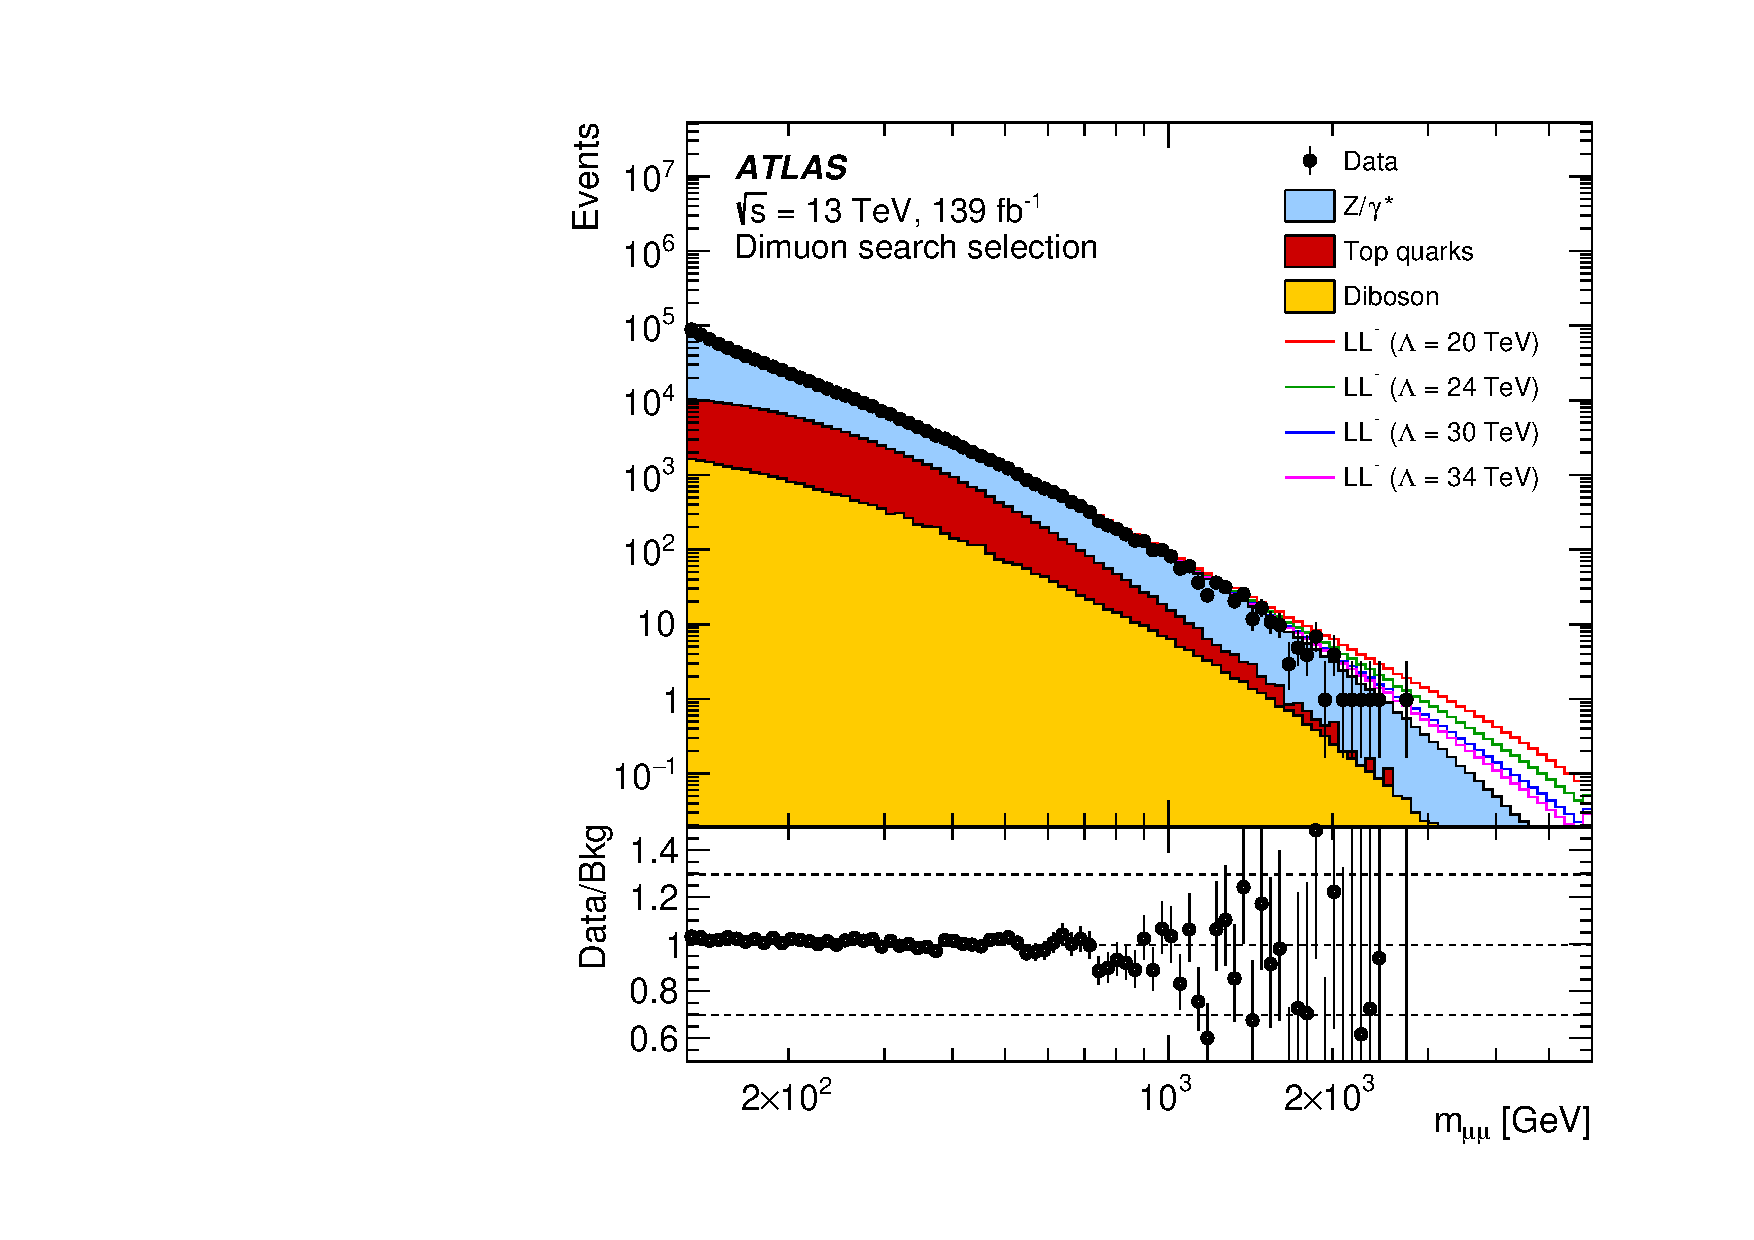
\includegraphics[width=1\textwidth]{figures/ci/dataMc/figaux_06a.pdf}
    \subcaption{}
\end{minipage}
\begin{minipage}[b]{.45\linewidth}
    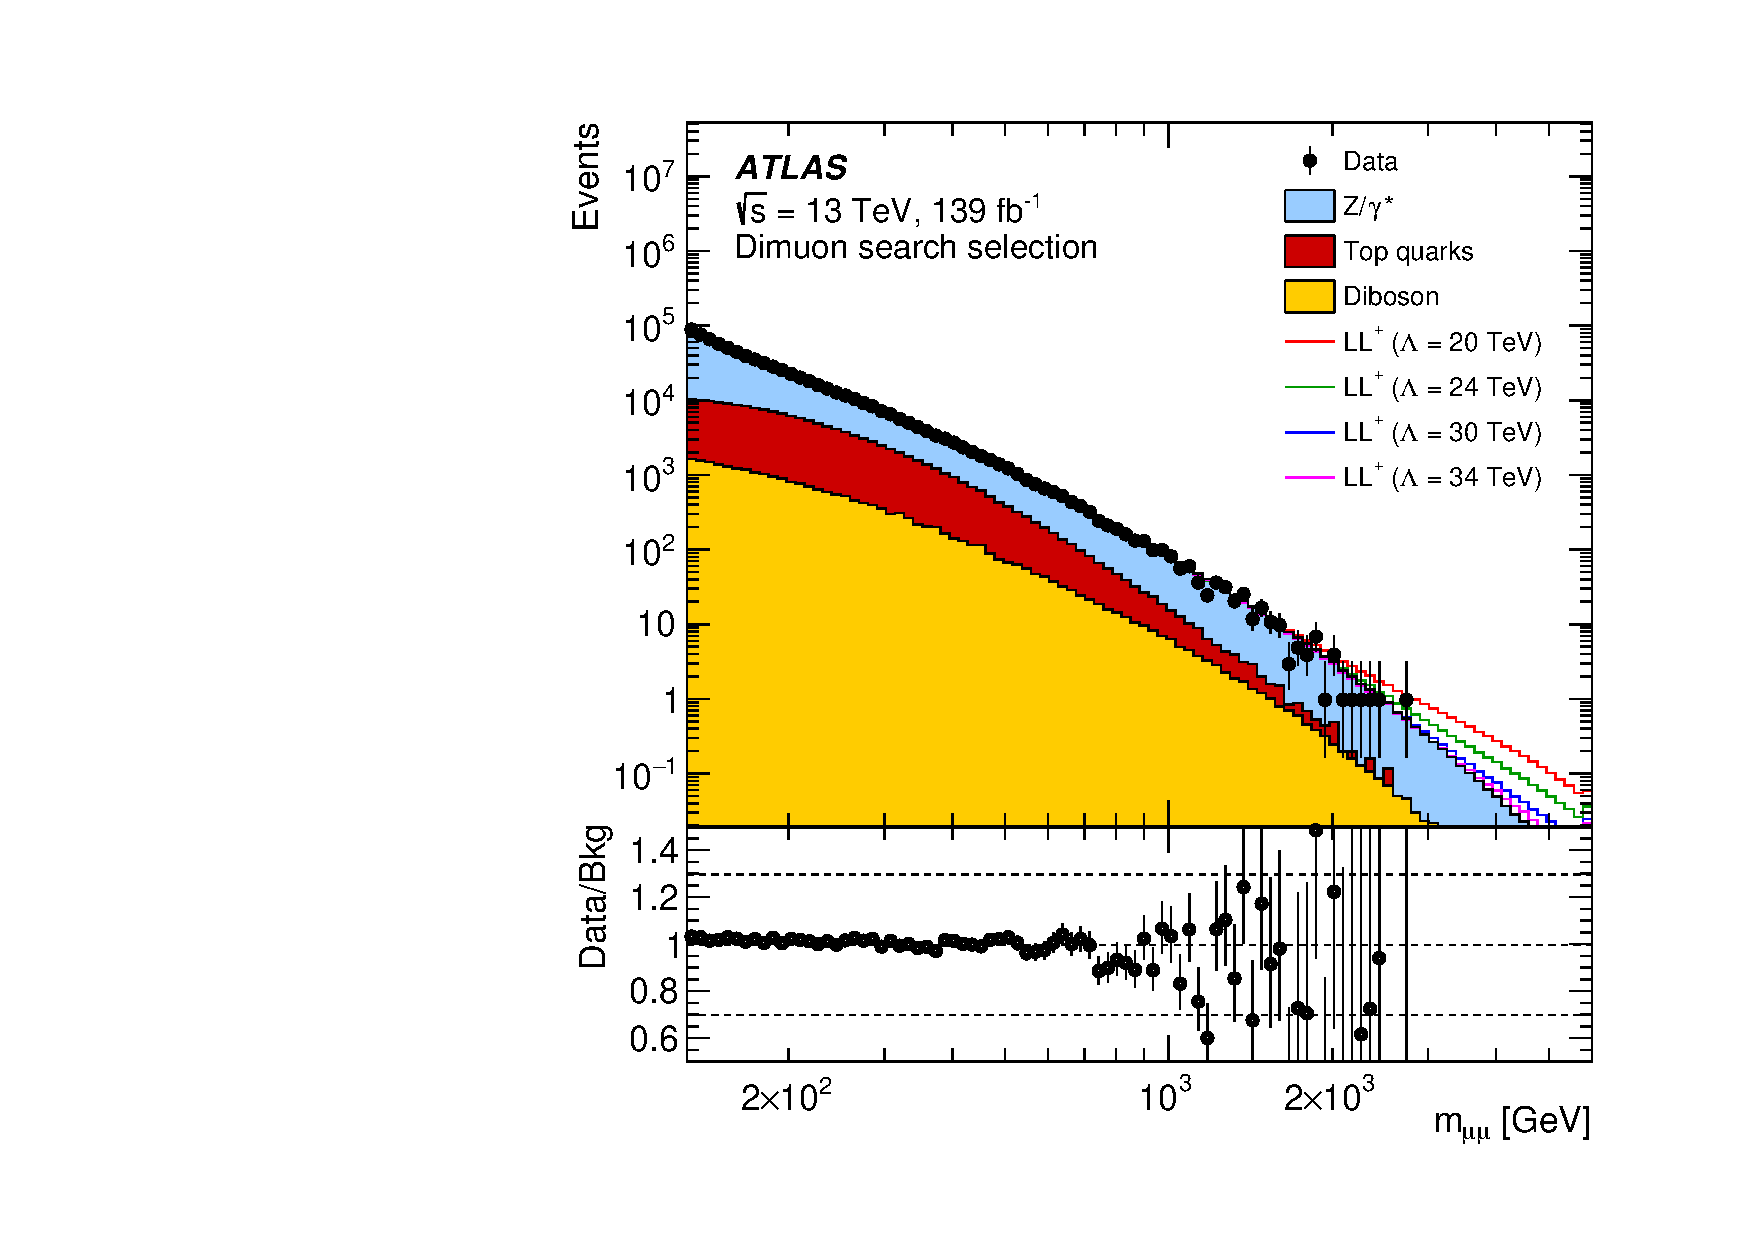
\includegraphics[width=1\textwidth]{figures/ci/dataMc/figaux_06b.pdf}
    \subcaption{}
\end{minipage}
\caption{Invariant-mass distributions in the $ee$ channel (top) and $\mu\mu$ channel (bottom). Plots on the left show selected constructive CI signal shapes imposed on top of the simulated distribution, while plots on the right show the same for destructive CI signal shapes.}
\label{fig:ciMassMcPlot}
\end{figure}
\clearpage
}

\afterpage{
\begin{figure}[h!]
\captionsetup[subfigure]{position=b}
\centering
 \begin{minipage}[b]{.45\linewidth}
    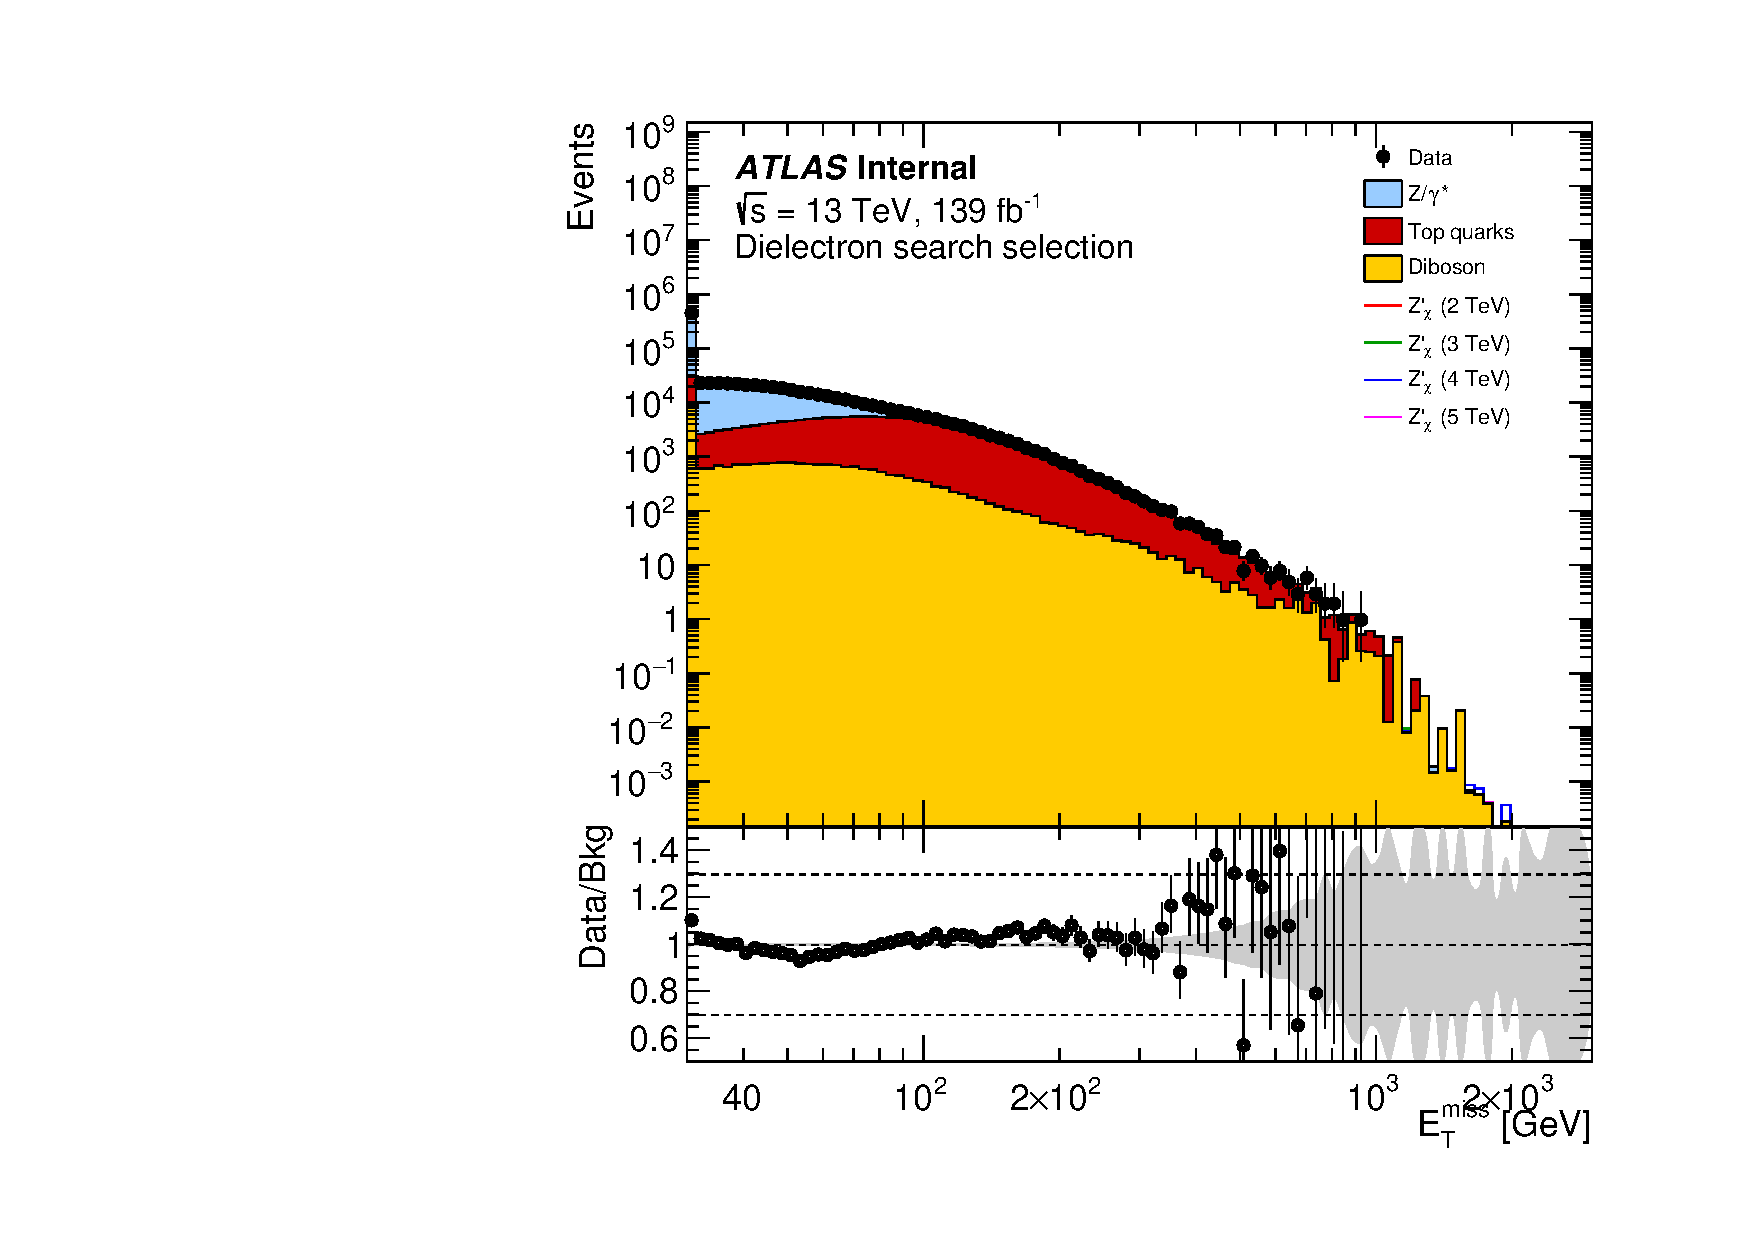
\includegraphics[width=1\textwidth]{figures/ci/dataMc/stacks_mc16e_2015-2018_ee_met_log100.pdf}
    \subcaption{}\label{fig:1a}
\end{minipage}
\begin{minipage}[b]{.45\linewidth}
    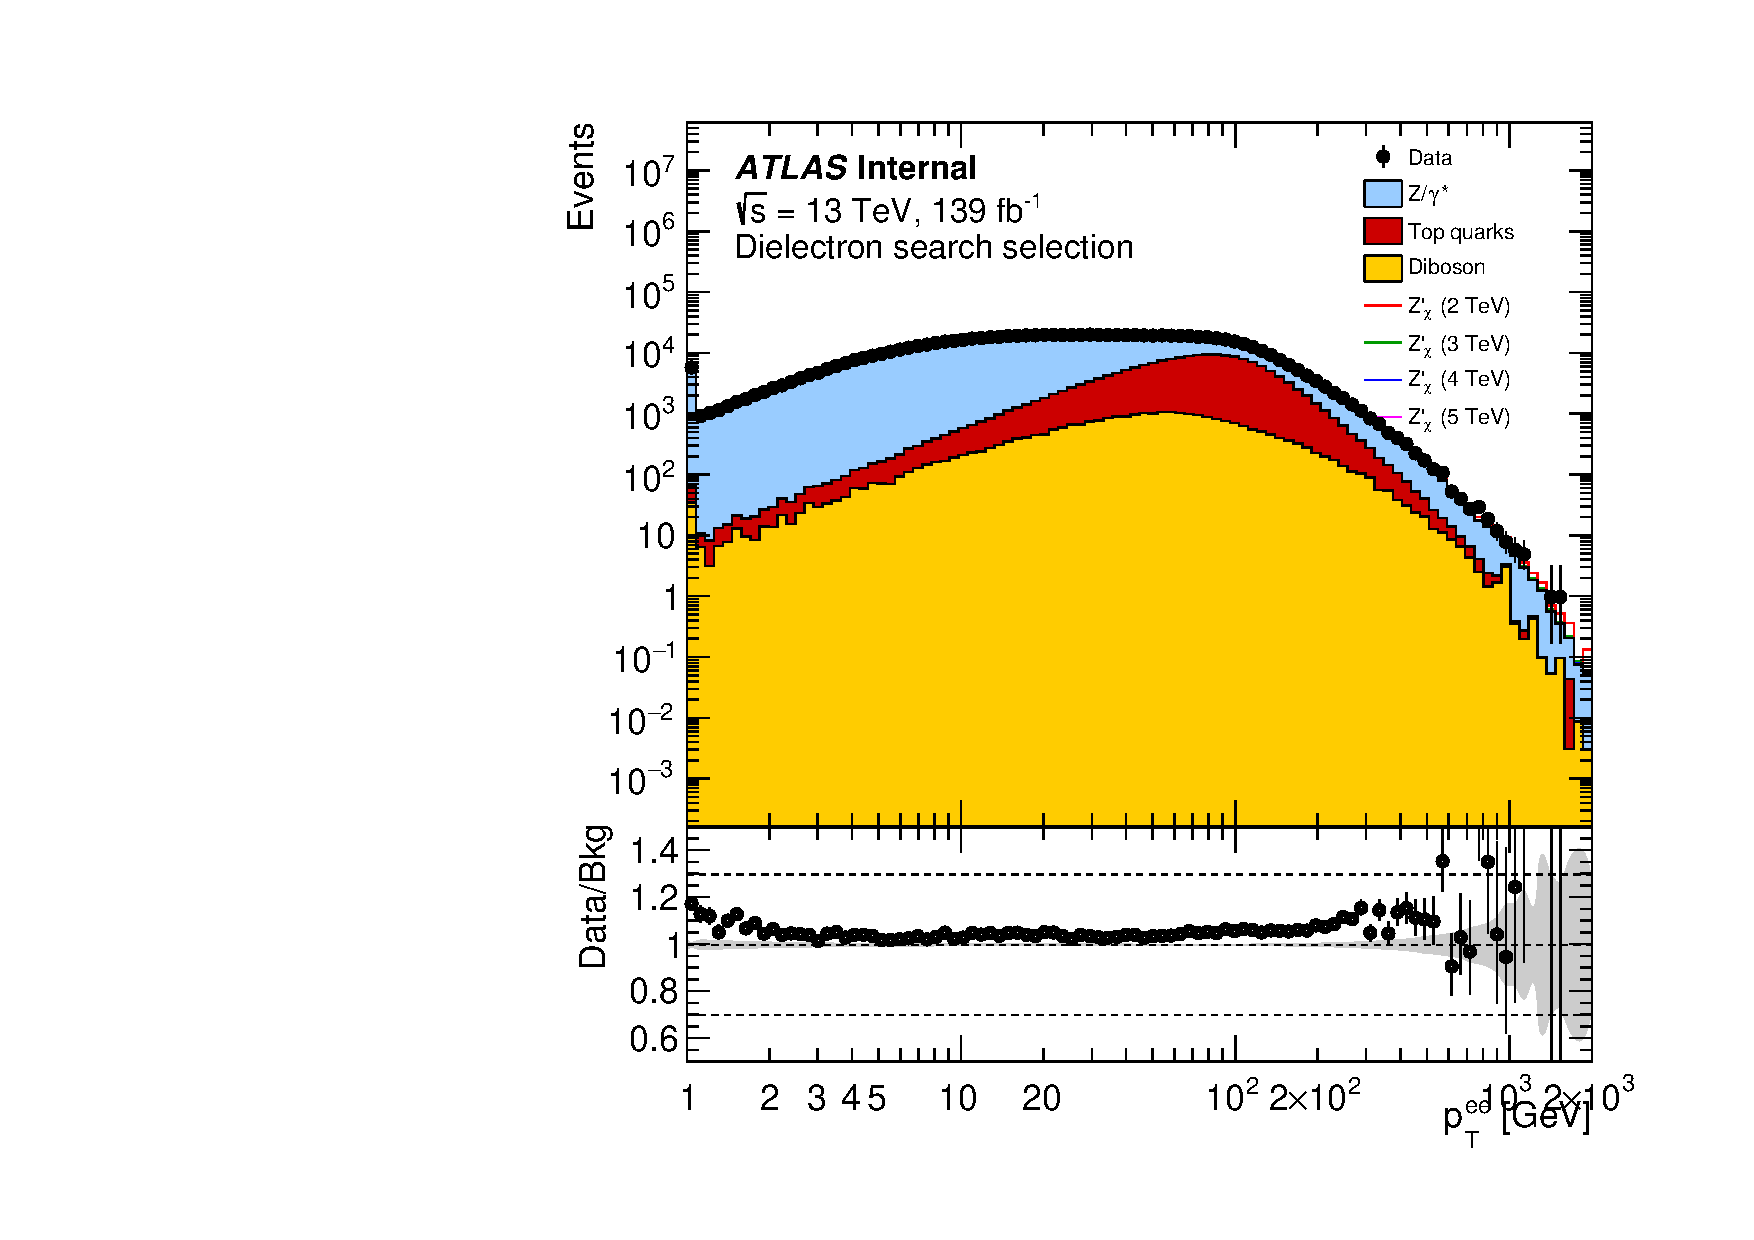
\includegraphics[width=1\textwidth]{figures/ci/dataMc/stacks_mc16e_2015-2018_ee_ptll_log100.pdf}
    \subcaption{}
\end{minipage} \\
\begin{minipage}[b]{.45\linewidth}
    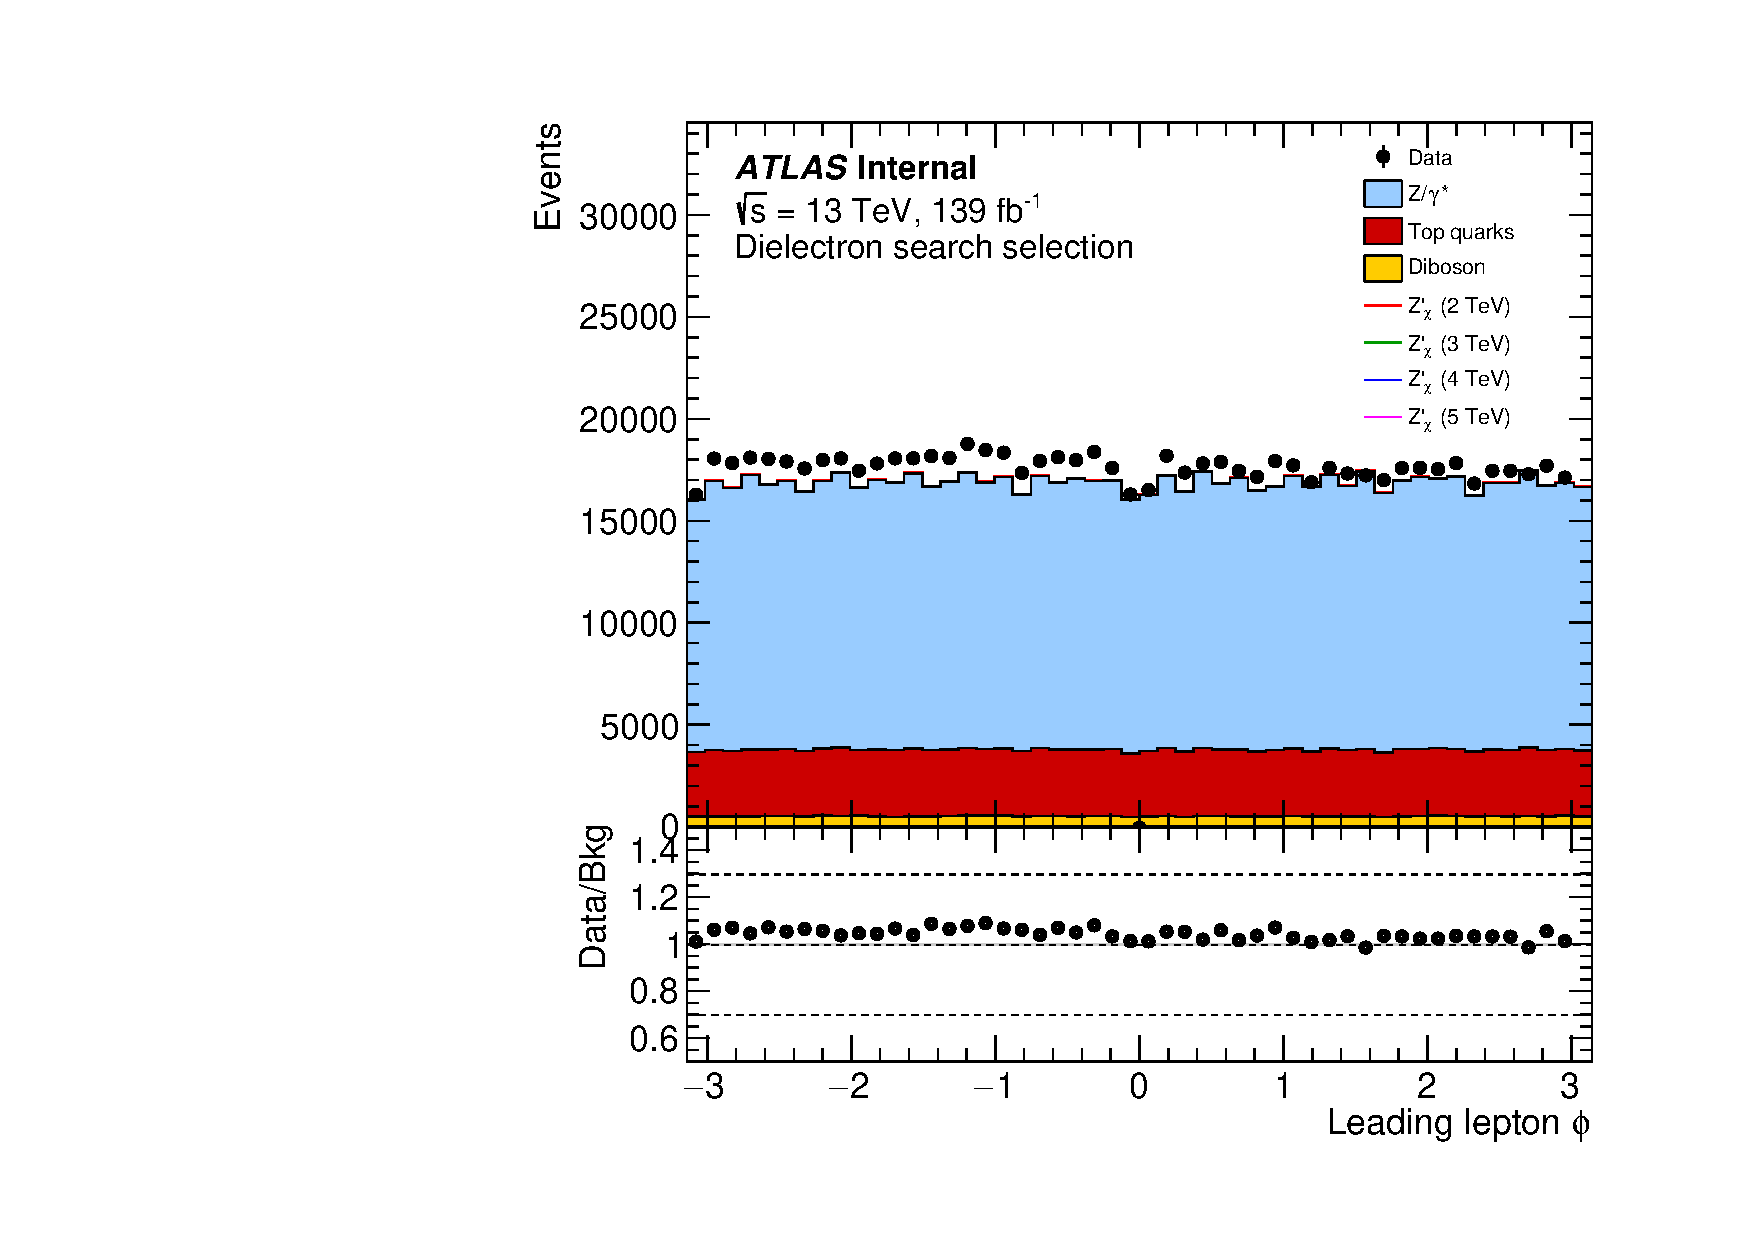
\includegraphics[width=1\textwidth]{figures/ci/dataMc/stacks_mc16e_2015-2018_ee_phi1.pdf}
    \subcaption{}
\end{minipage}
\begin{minipage}[b]{.45\linewidth}
    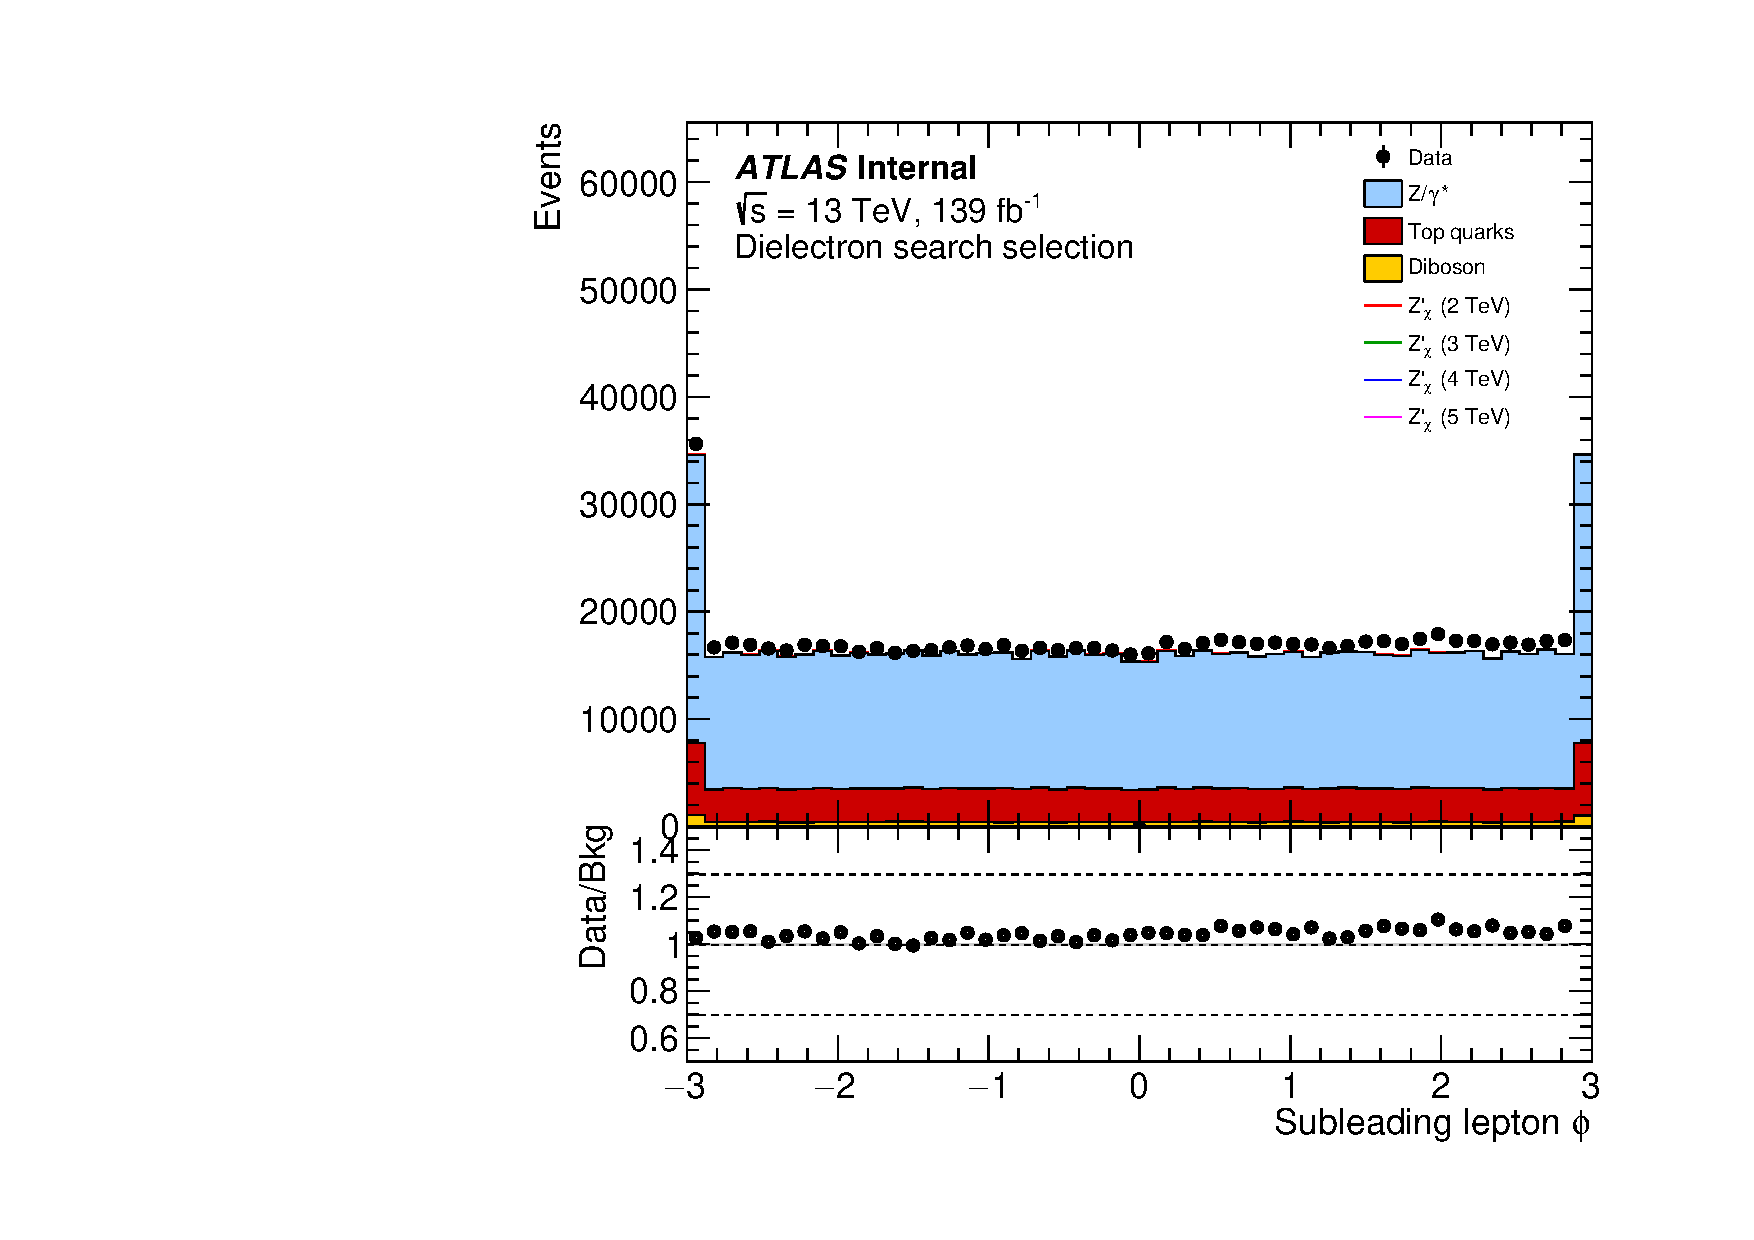
\includegraphics[width=1\textwidth]{figures/ci/dataMc/stacks_mc16e_2015-2018_ee_phi2.pdf}
    \subcaption{}
\end{minipage}
\caption{Kinematic distributions in the $ee$ channel. (a) $E_T^\text{miss}$, (b) dielectron \pt, leading electron $\phi$, and subleading electron $\phi$.}
\label{fig:}
\end{figure}
\clearpage
}

\afterpage{
\begin{figure}[h!]
\captionsetup[subfigure]{position=b}
\centering
\begin{minipage}[b]{.45\linewidth}
    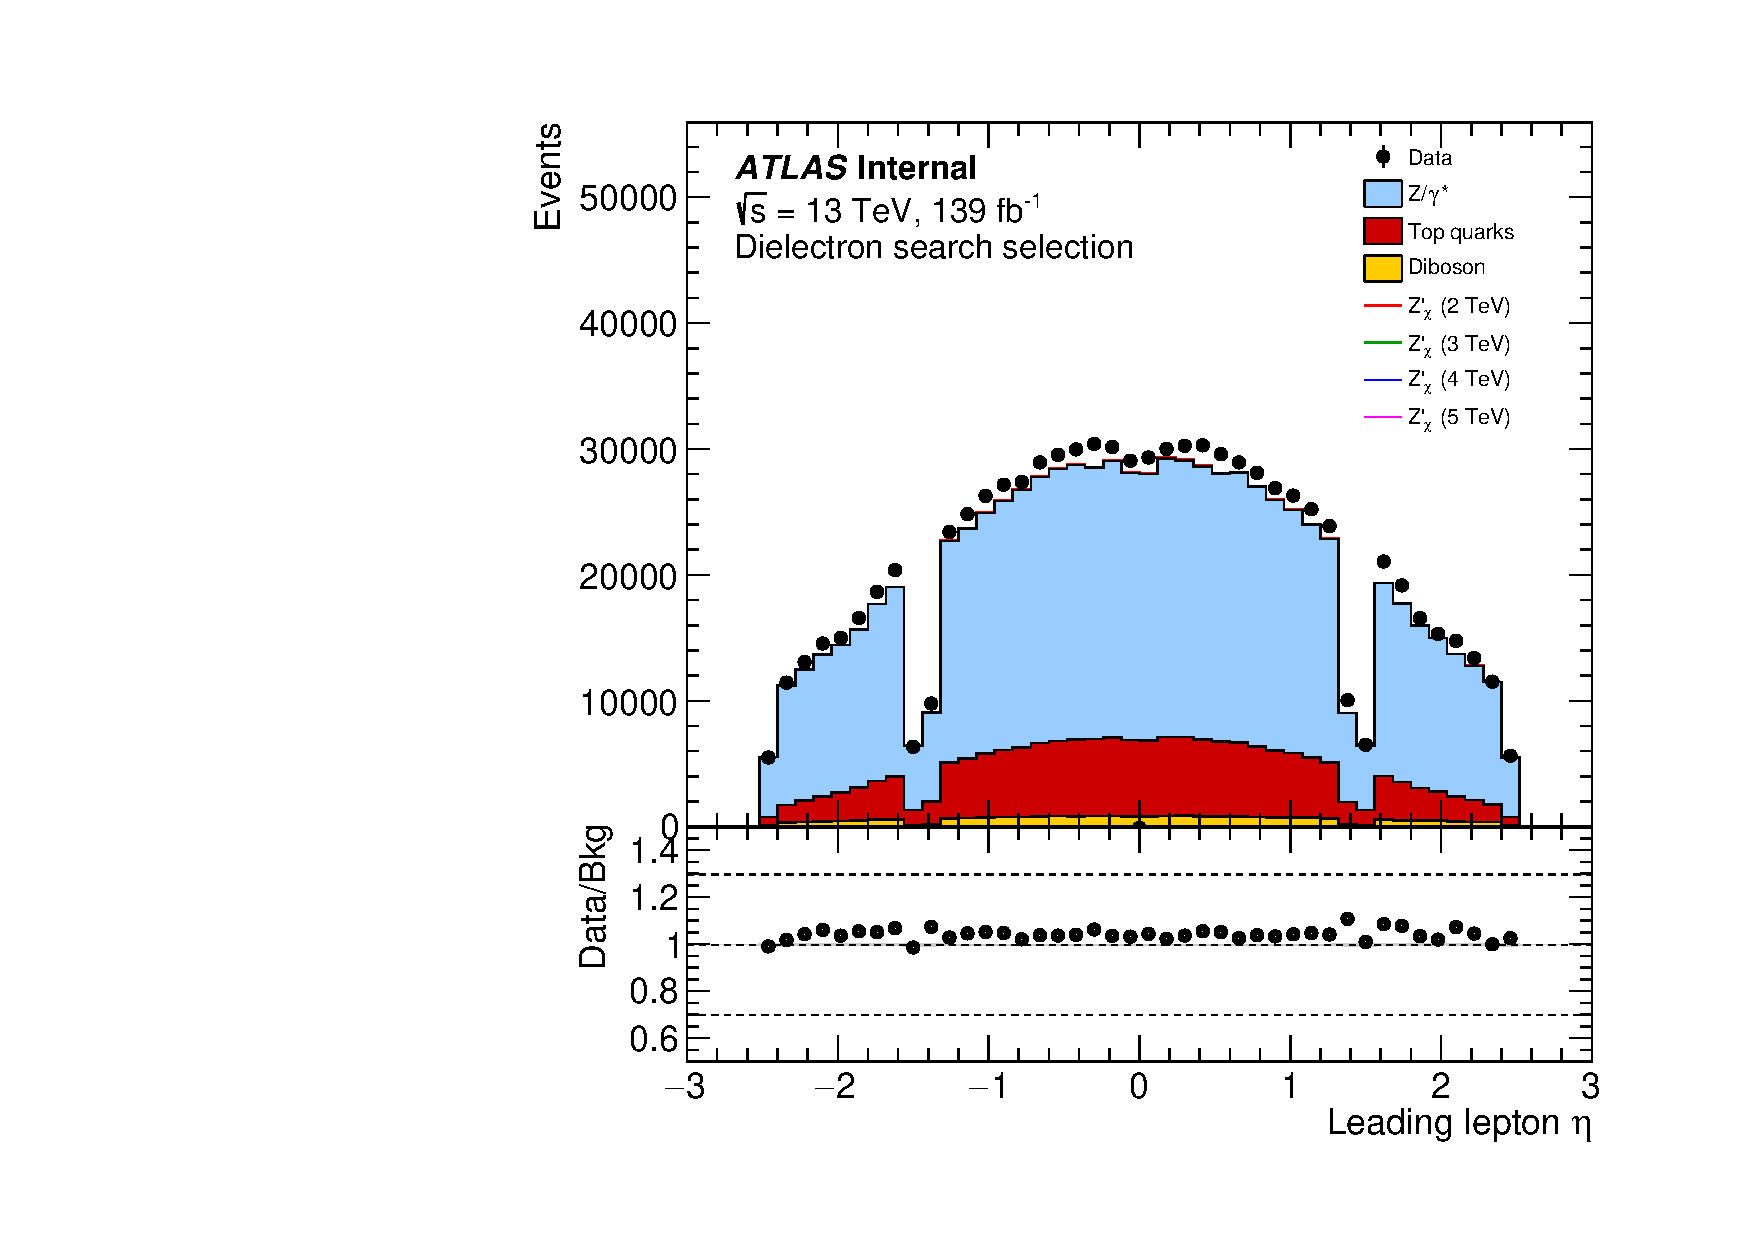
\includegraphics[width=1\textwidth]{figures/ci/dataMc/stacks_mc16e_2015-2018_ee_eta1.pdf}
    \subcaption{}
\end{minipage} 
\begin{minipage}[b]{.45\linewidth}
    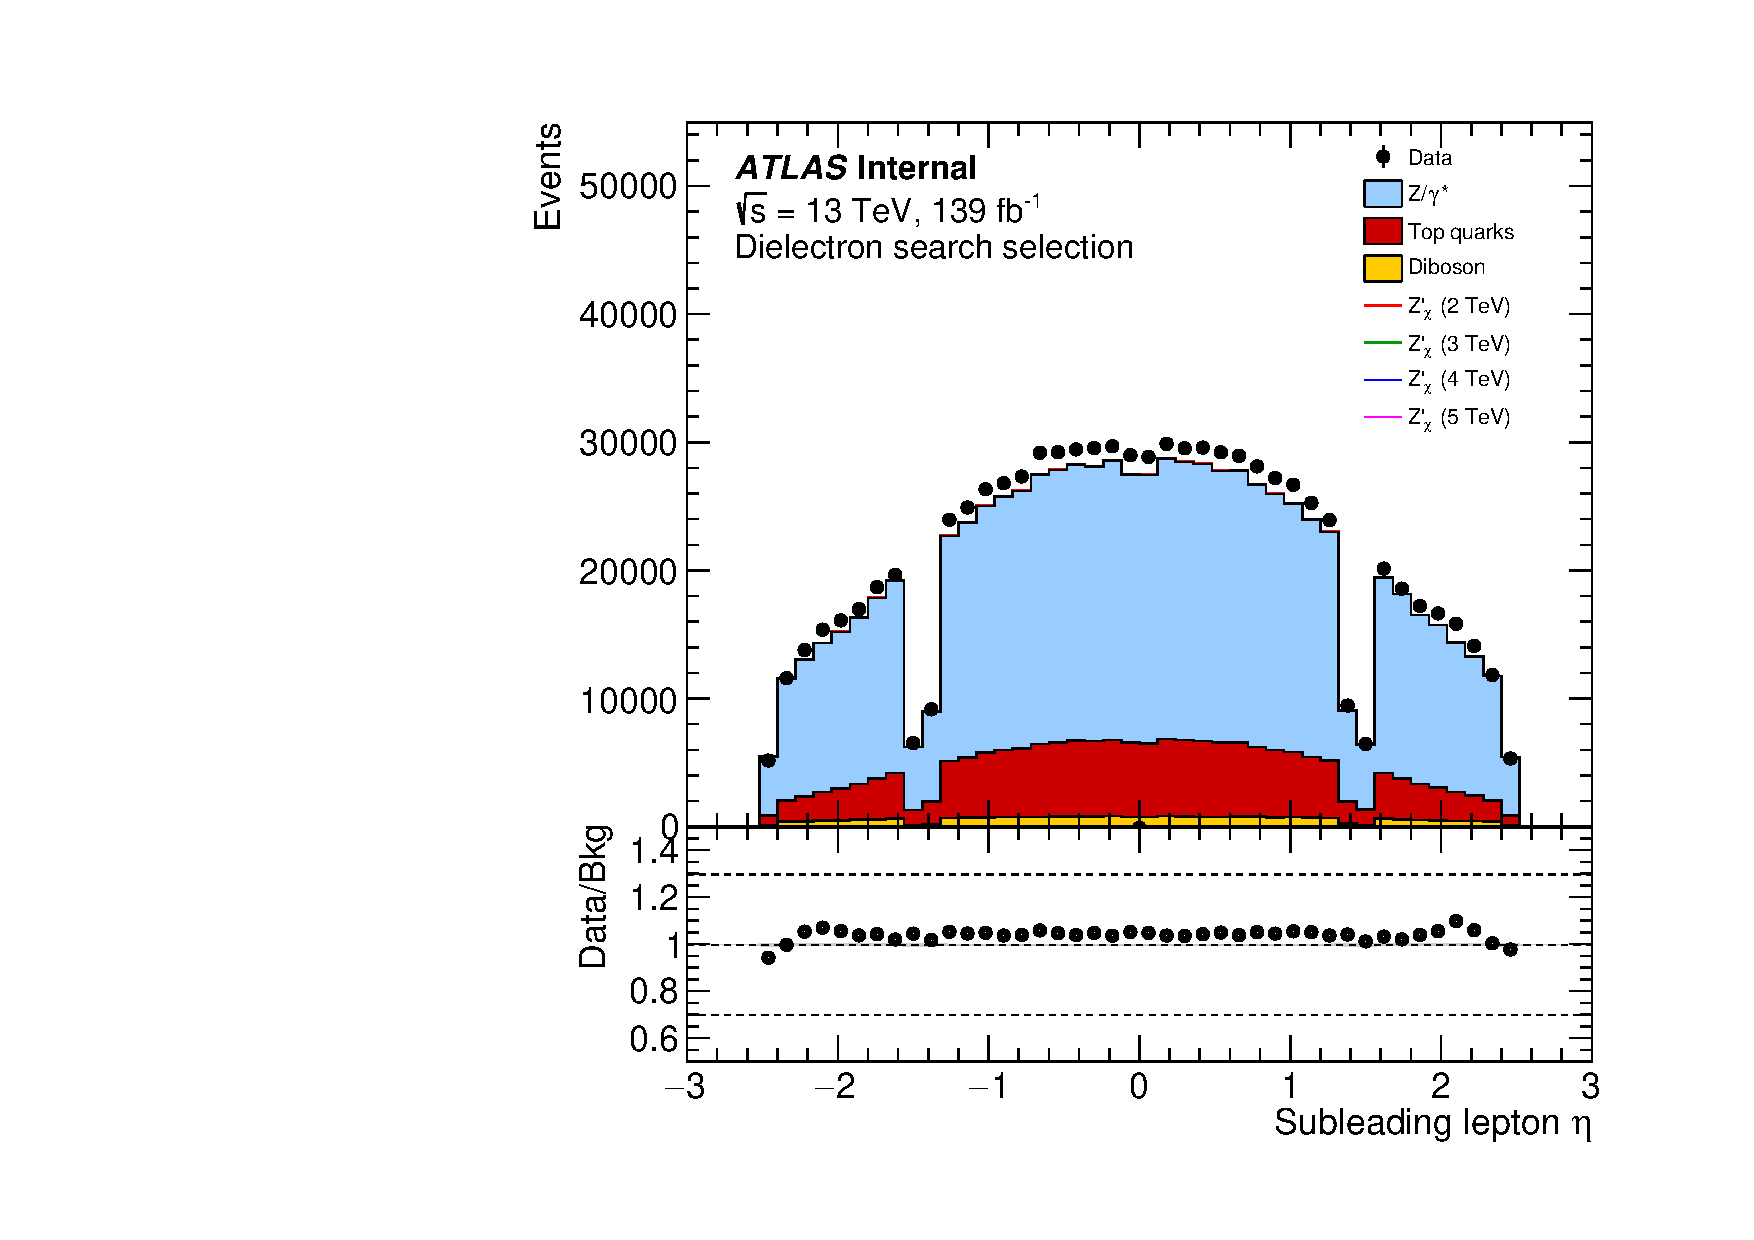
\includegraphics[width=1\textwidth]{figures/ci/dataMc/stacks_mc16e_2015-2018_ee_eta2.pdf}
    \subcaption{}
\end{minipage}\\
\begin{minipage}[b]{.45\linewidth}
    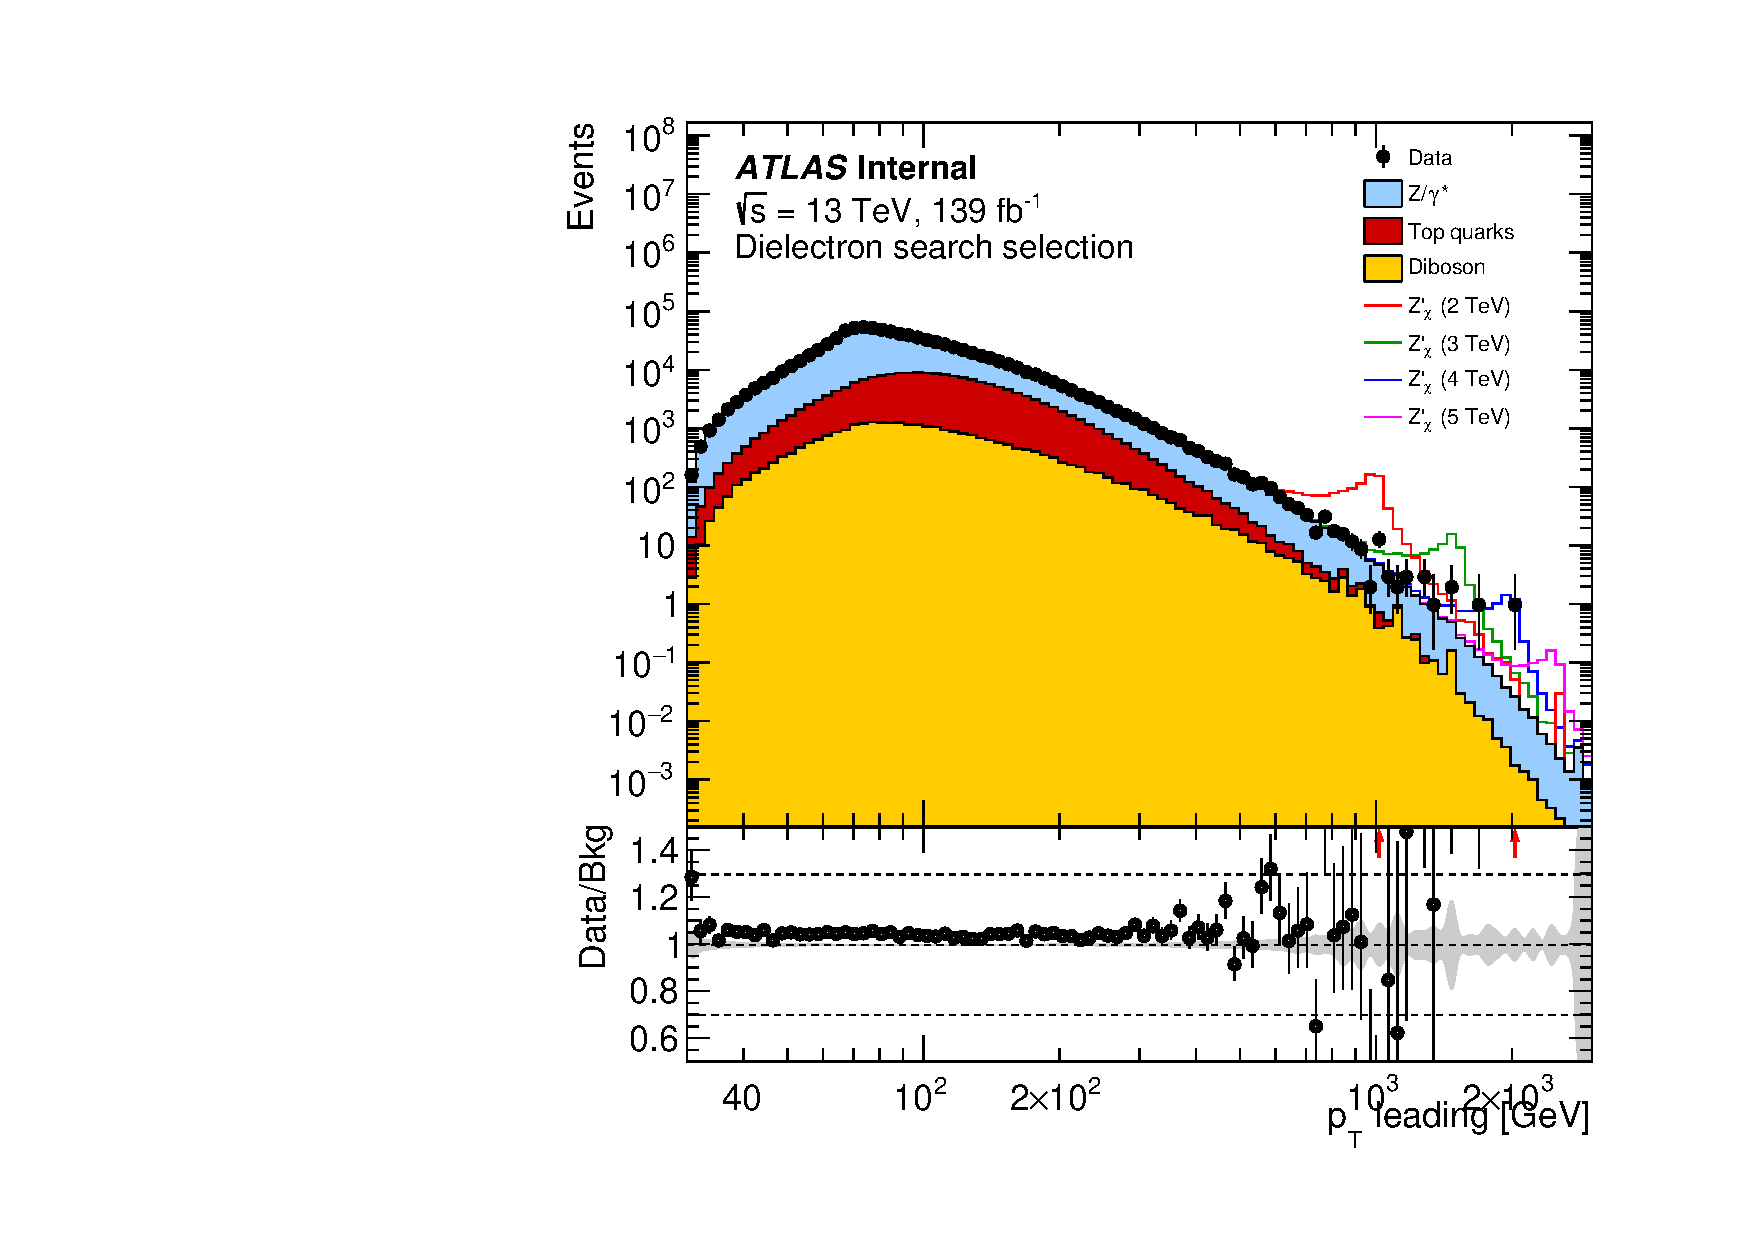
\includegraphics[width=1\textwidth]{figures/ci/dataMc/stacks_mc16e_2015-2018_ee_pt1_log100.pdf}
    \subcaption{}
\end{minipage}
\begin{minipage}[b]{.45\linewidth}
    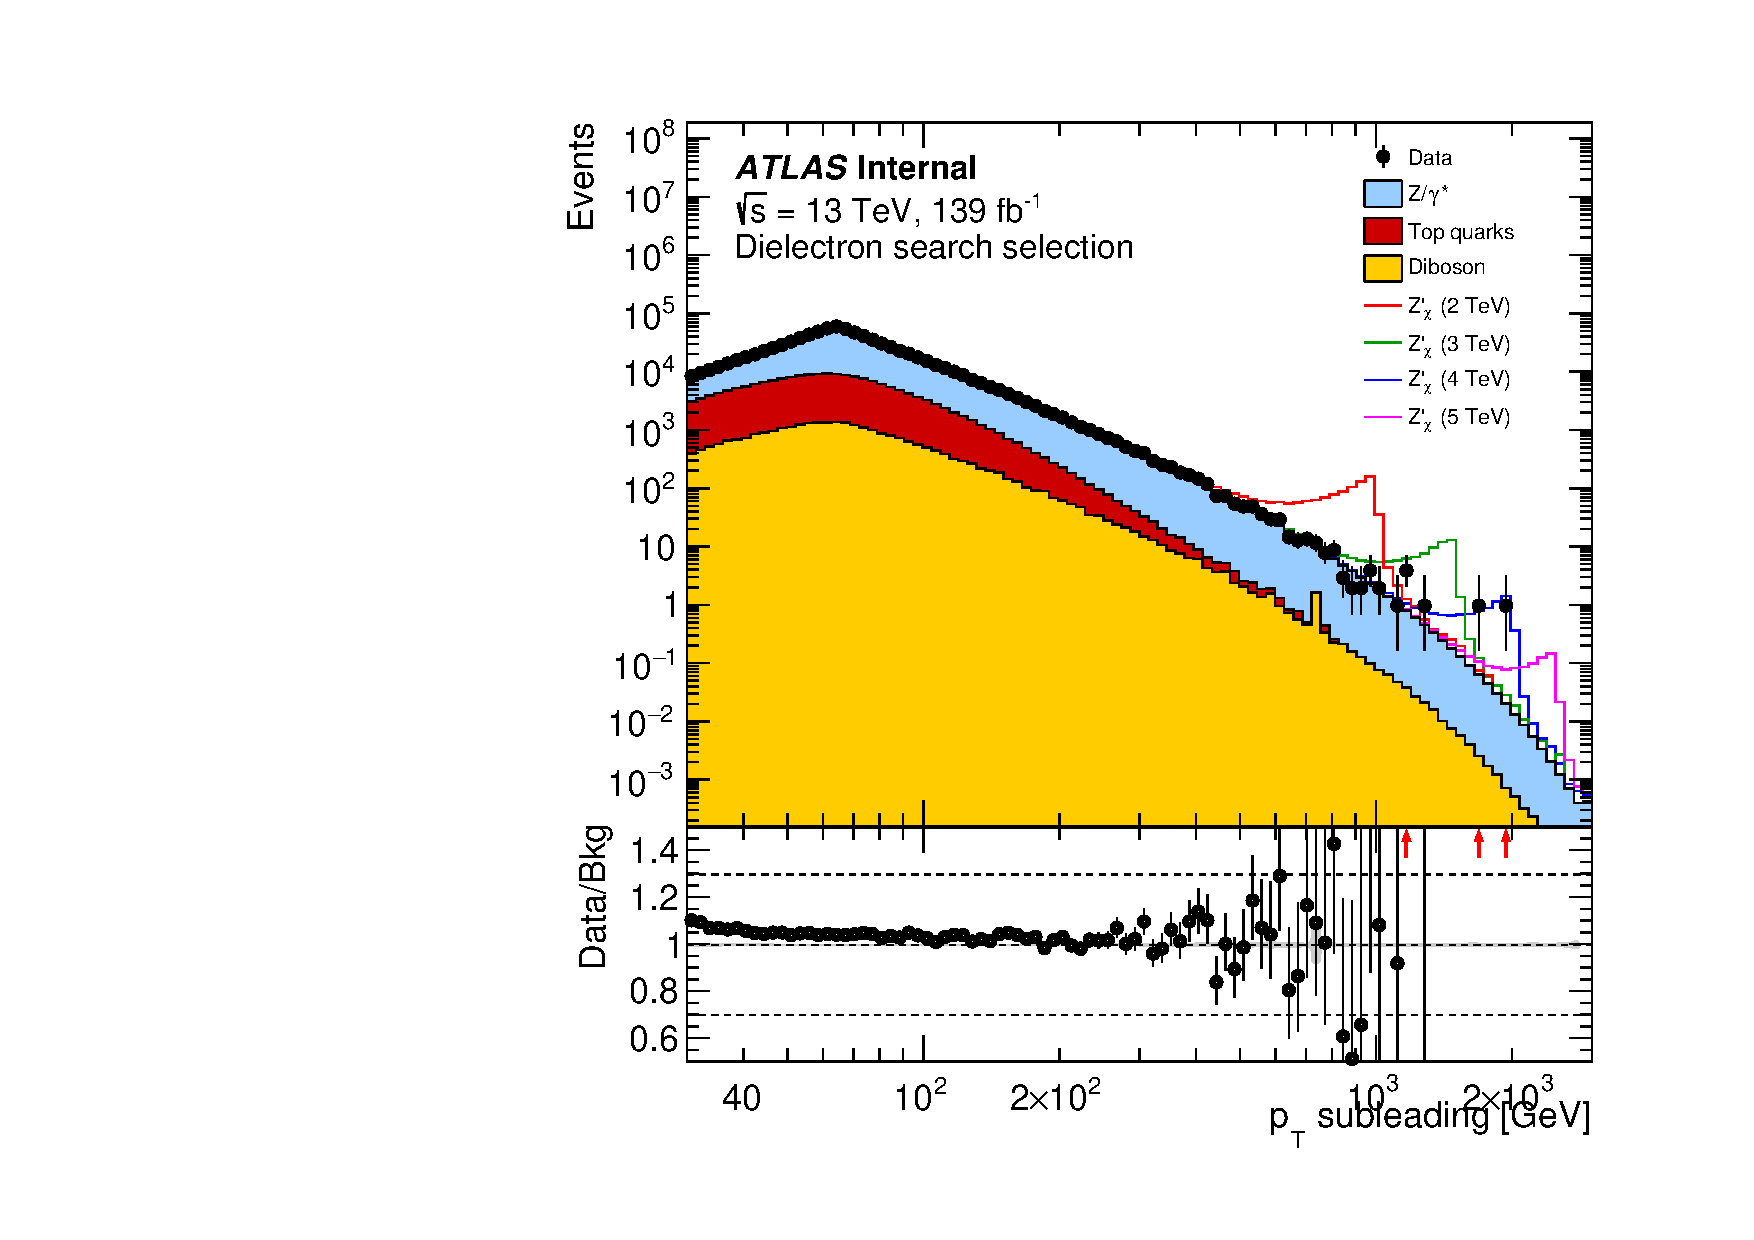
\includegraphics[width=1\textwidth]{figures/ci/dataMc/stacks_mc16e_2015-2018_ee_pt2_log100.pdf}
    \subcaption{}
\end{minipage}
\caption{Kinematic distributions in the $ee$ channel. (a) leading electron $\eta$, (b) subleading electron $\eta$, leading electron \pt, and subleading electron \pt.}
\label{fig:}
\end{figure}
\clearpage
}

\afterpage{
\begin{figure}[h!]
\captionsetup[subfigure]{position=b}
\centering
 \begin{minipage}[b]{.45\linewidth}
    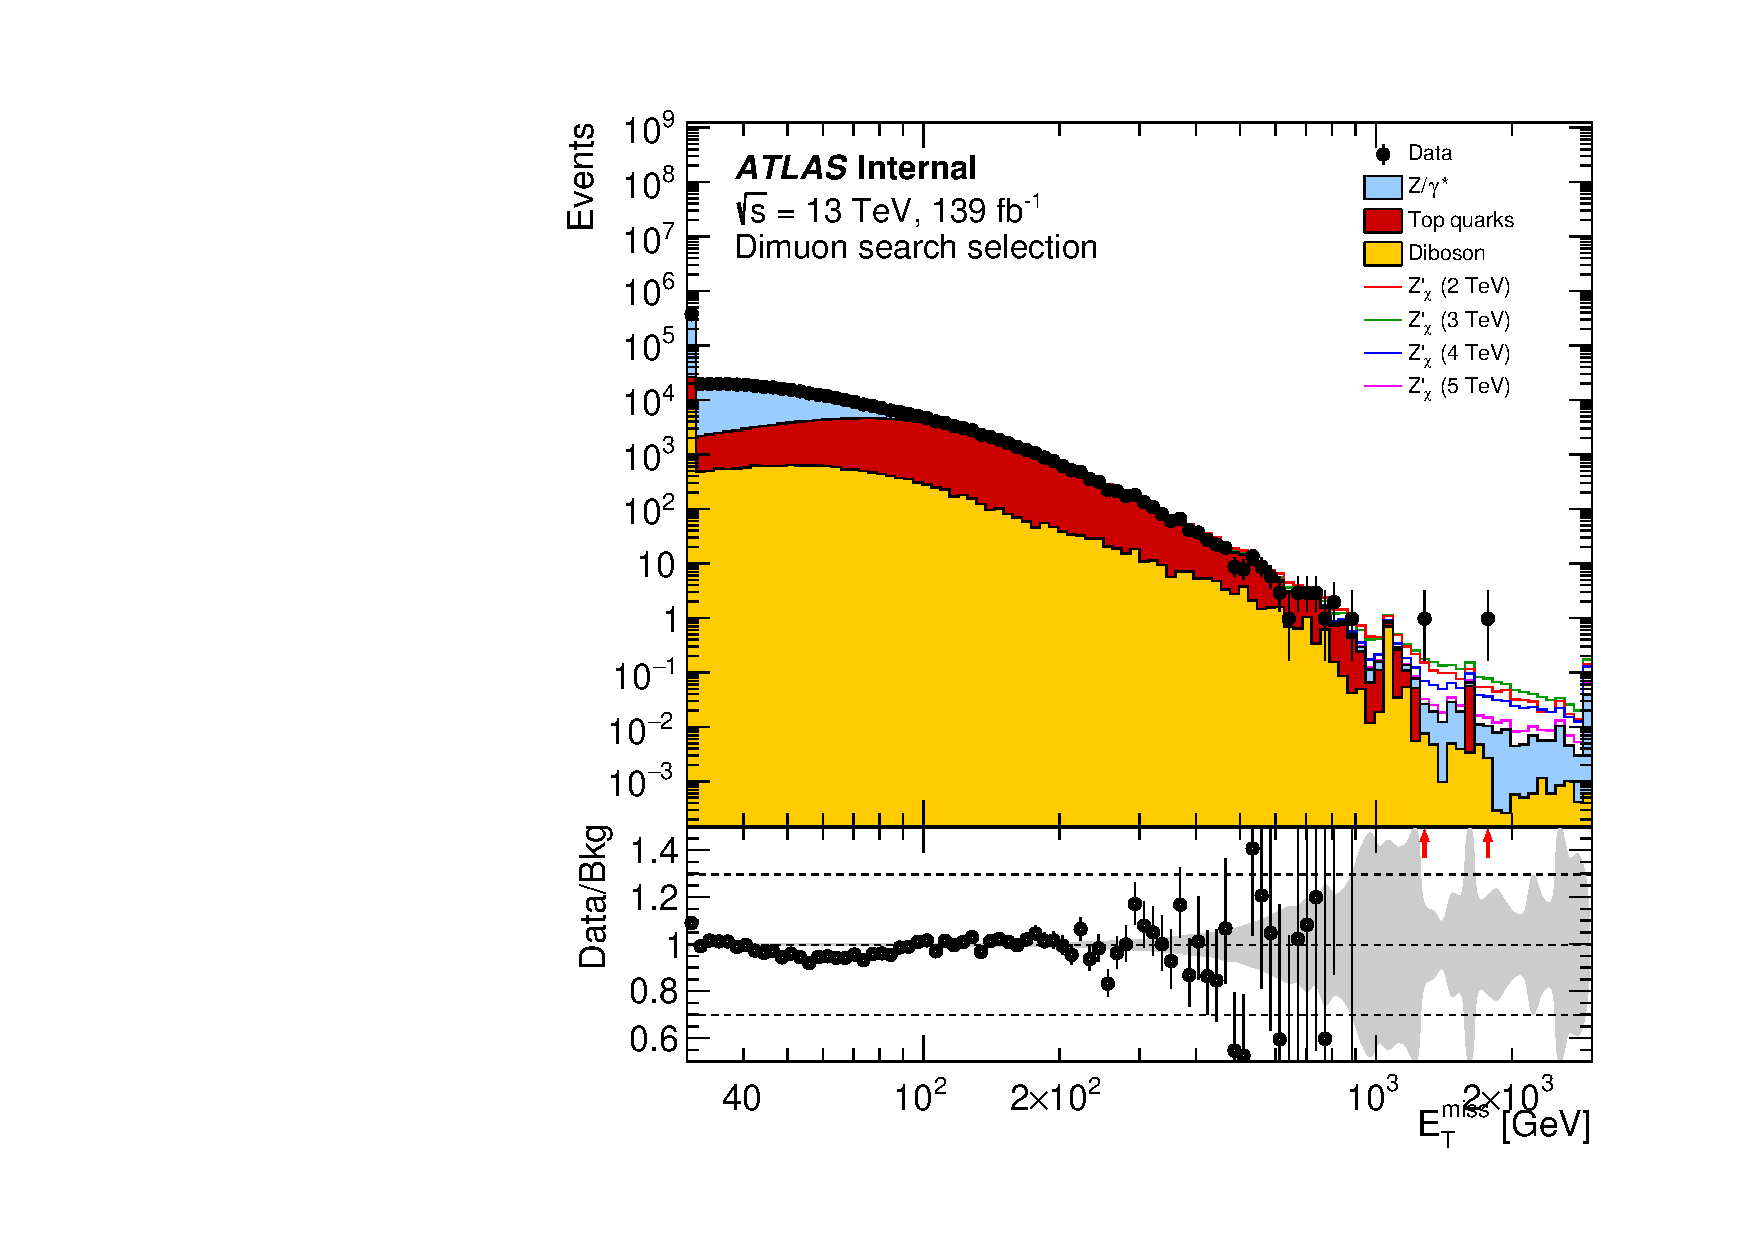
\includegraphics[width=1\textwidth]{figures/ci/dataMc/stacks_mc16e_2015-2018_uu_met_log100.pdf}
    \subcaption{}\label{fig:1a}
\end{minipage}
\begin{minipage}[b]{.45\linewidth}
    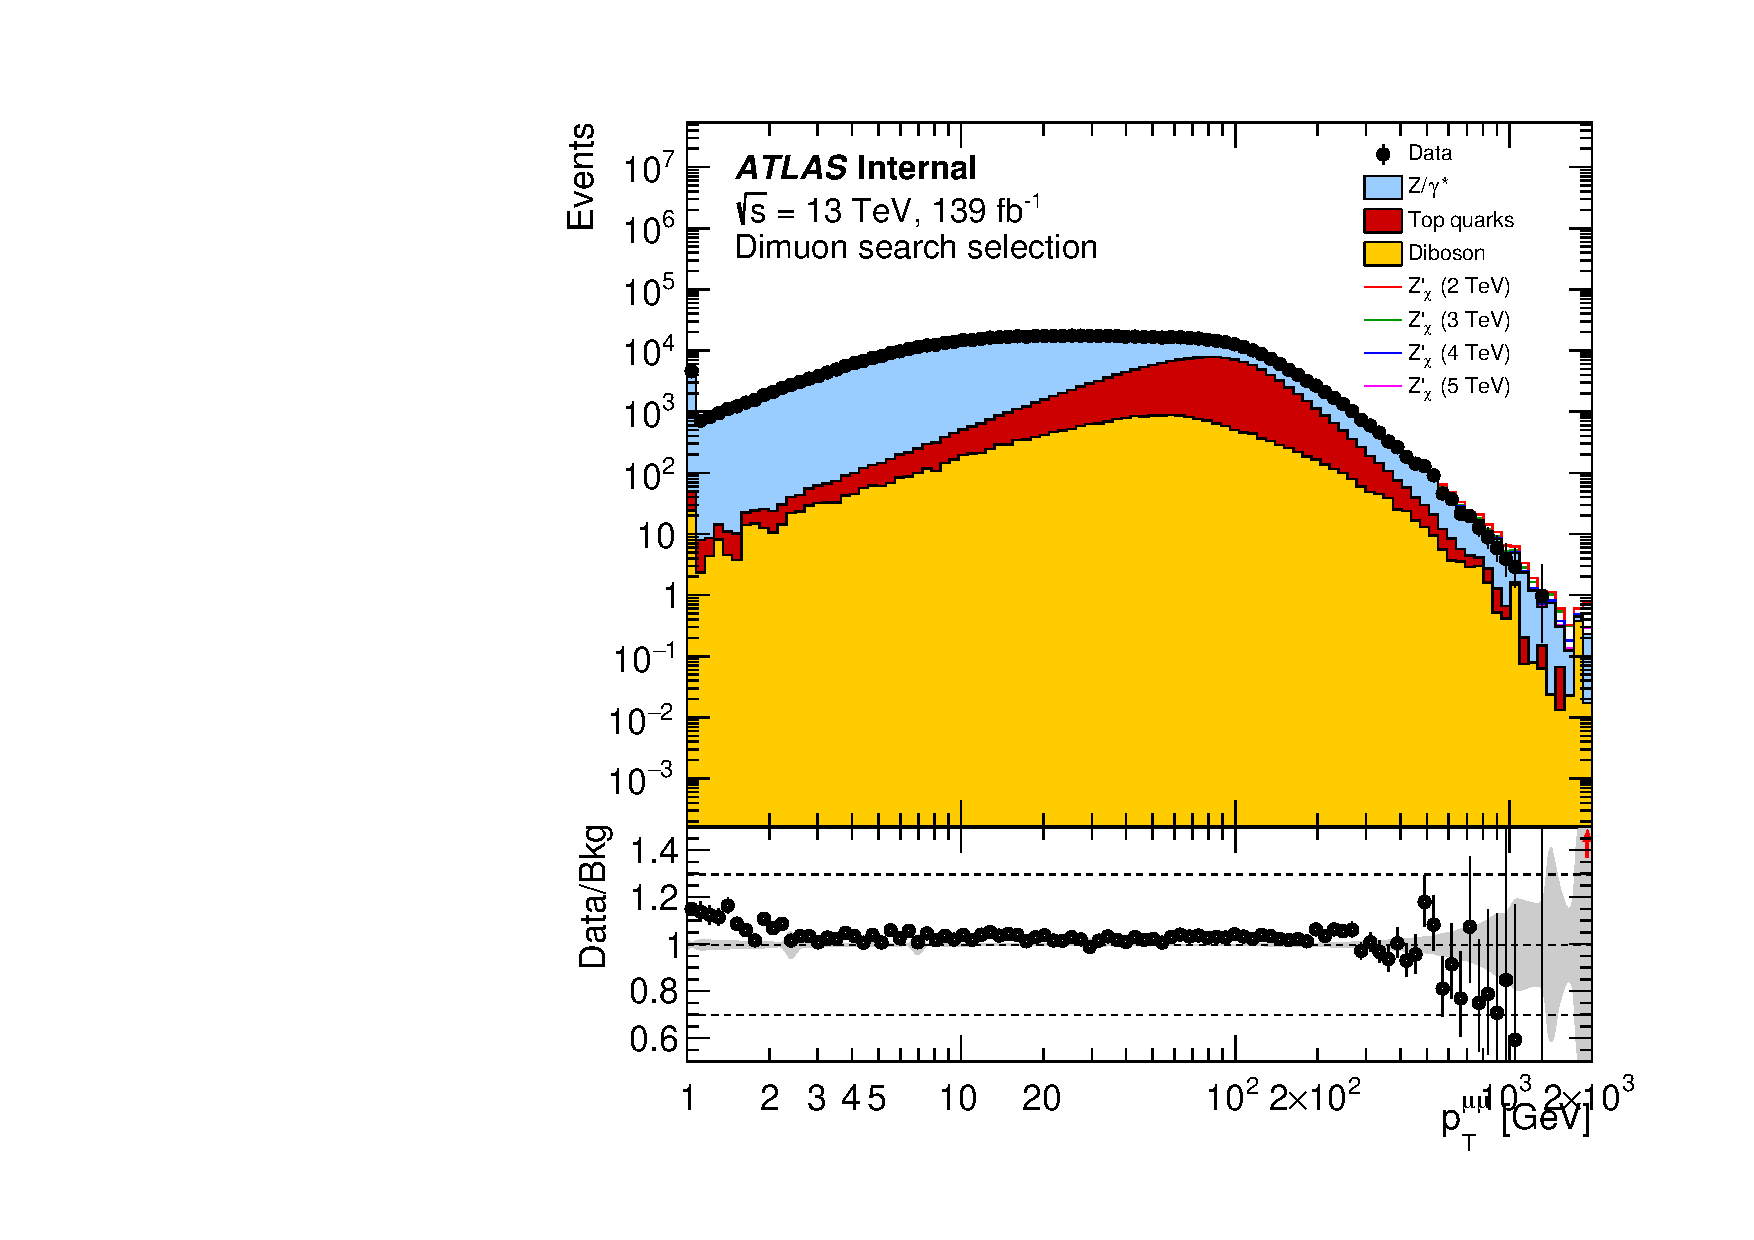
\includegraphics[width=1\textwidth]{figures/ci/dataMc/stacks_mc16e_2015-2018_uu_ptll_log100.pdf}
    \subcaption{}
\end{minipage} \\
\begin{minipage}[b]{.45\linewidth}
    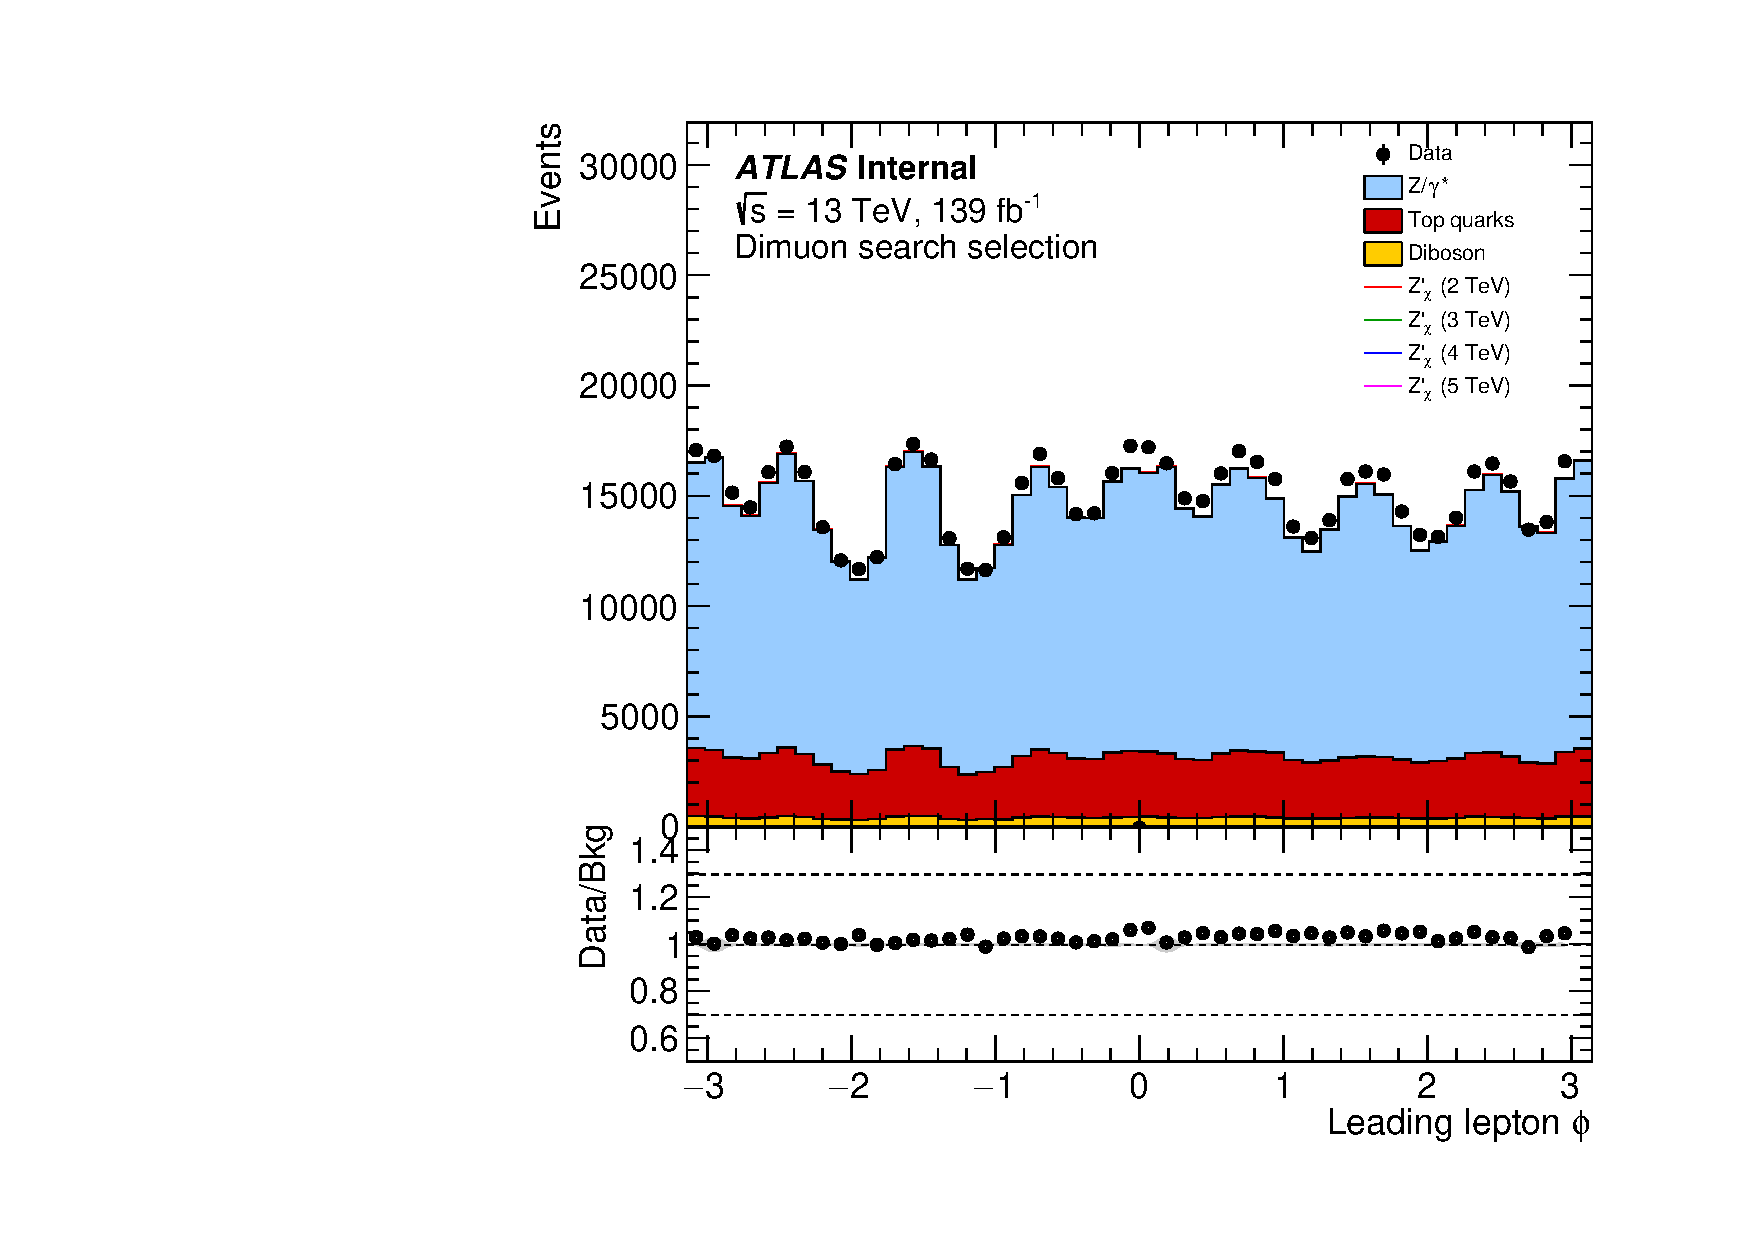
\includegraphics[width=1\textwidth]{figures/ci/dataMc/stacks_mc16e_2015-2018_uu_phi1.pdf}
    \subcaption{}
\end{minipage}
\begin{minipage}[b]{.45\linewidth}
    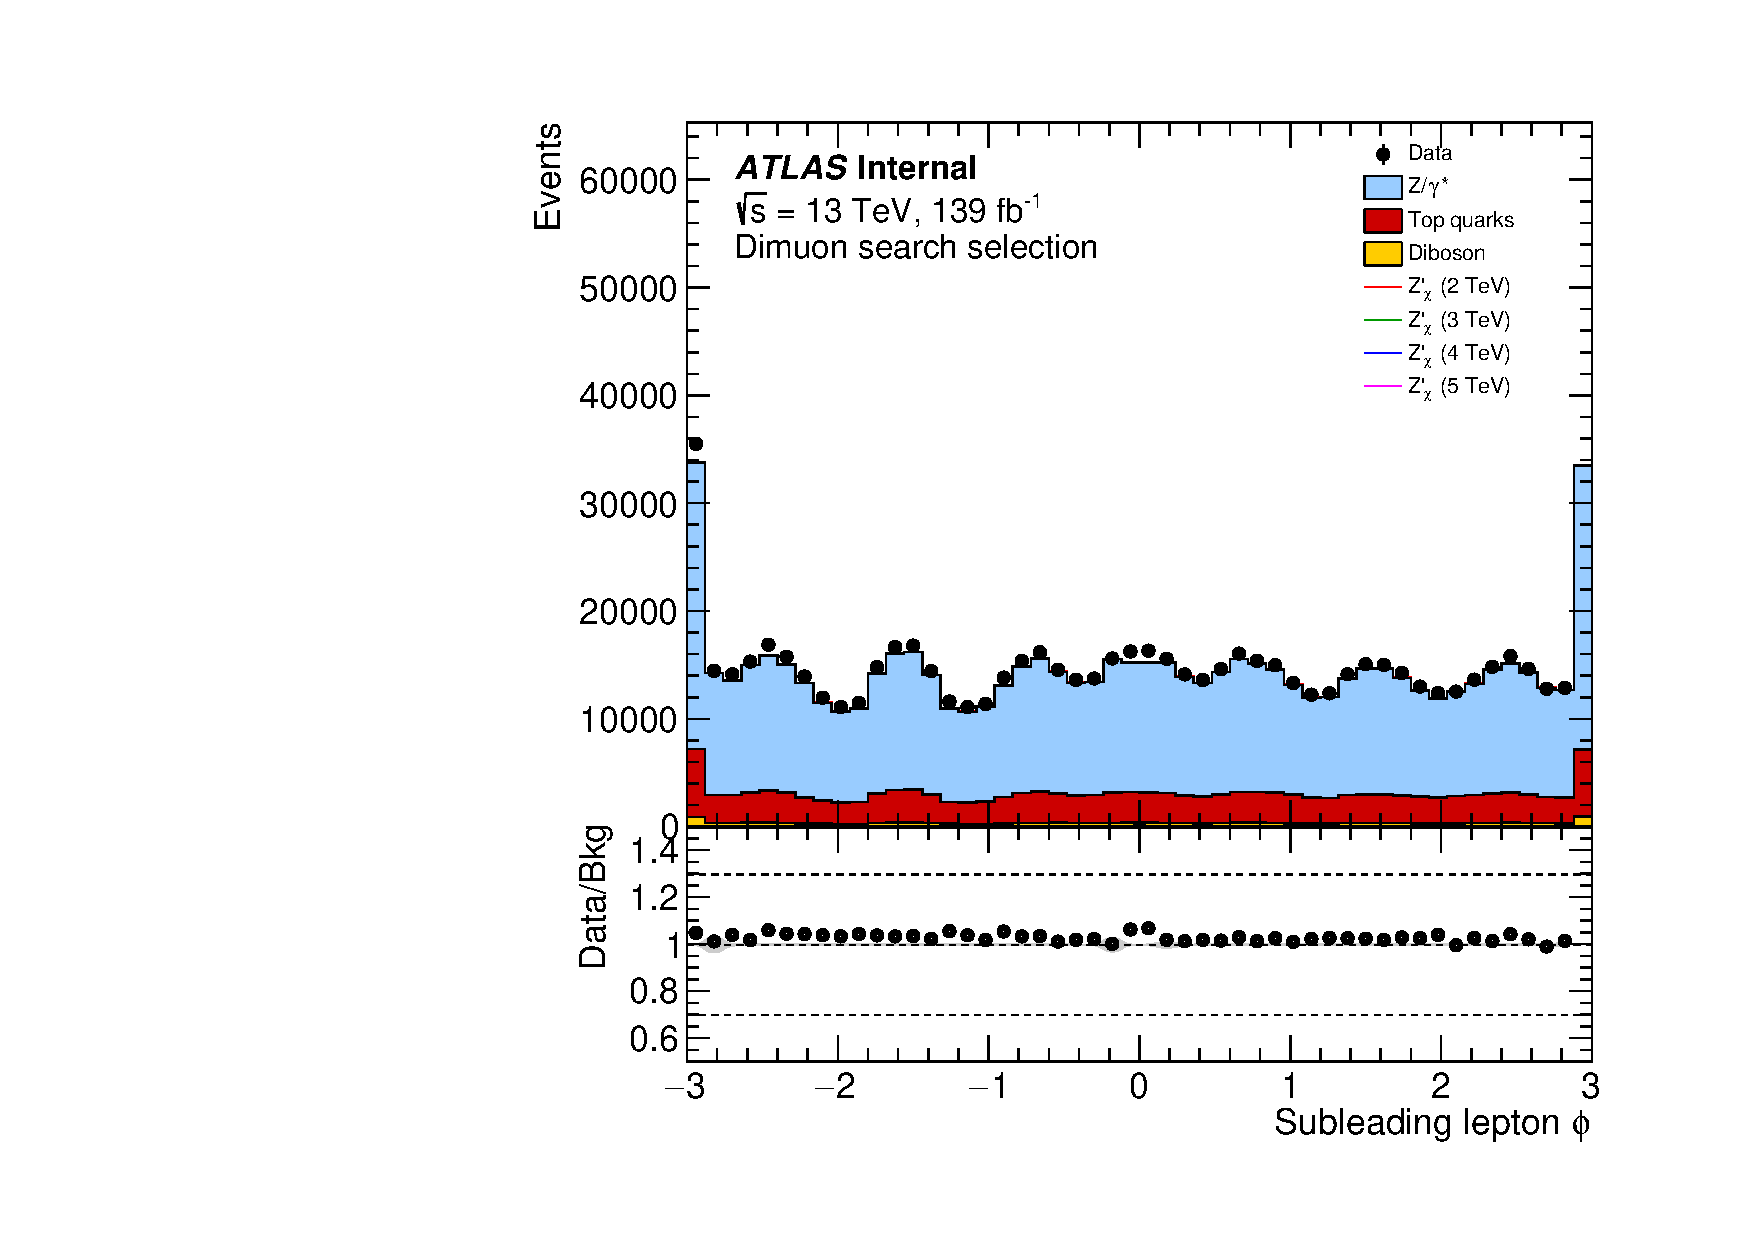
\includegraphics[width=1\textwidth]{figures/ci/dataMc/stacks_mc16e_2015-2018_uu_phi2.pdf}
    \subcaption{}
\end{minipage}
\caption{Kinematic distributions in the $\mu\mu$ channel. (a) $E_T^\text{miss}$, (b) dielectron \pt, leading muon $\phi$, and subleading muon $\phi$.}
\label{fig:}
\end{figure}
\clearpage
}

\afterpage{
\begin{figure}[h!]
\captionsetup[subfigure]{position=b}
\centering
\begin{minipage}[b]{.45\linewidth}
    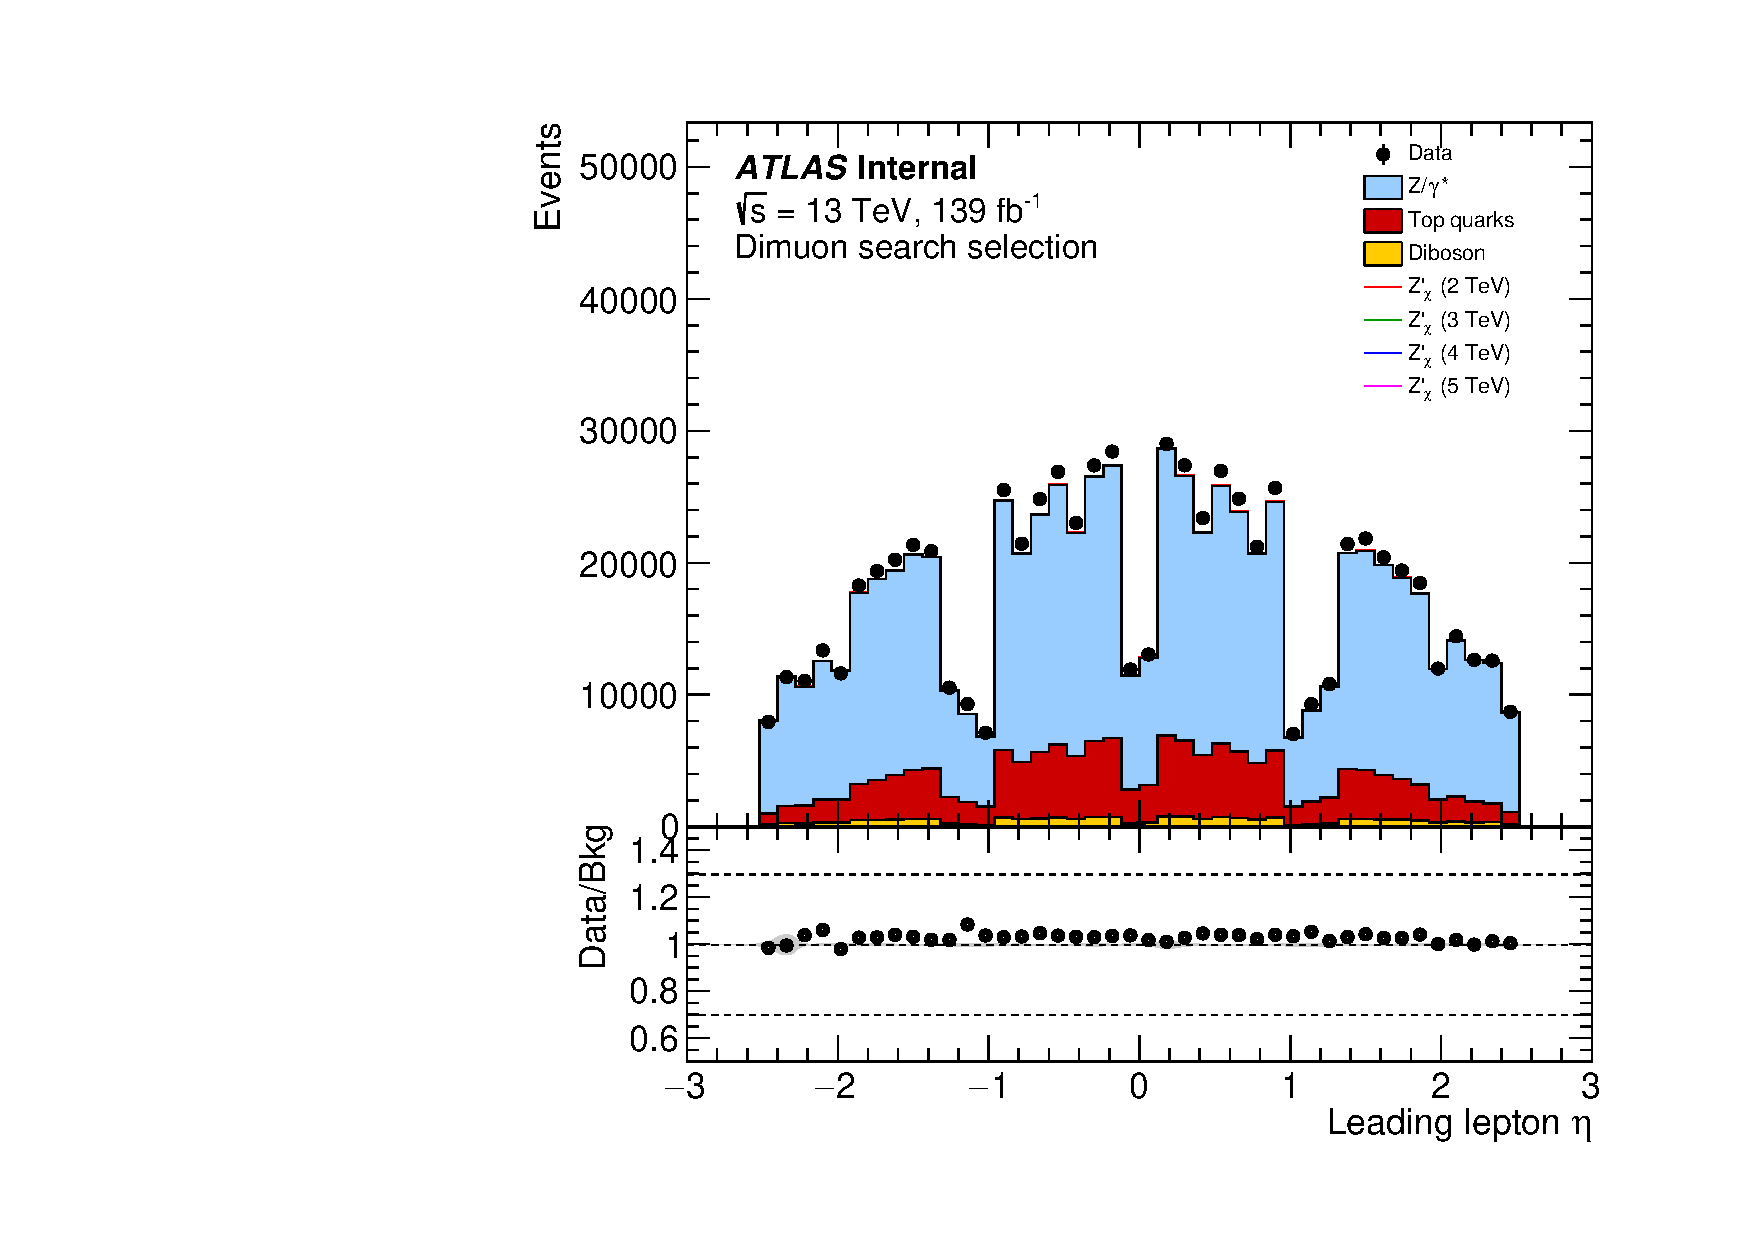
\includegraphics[width=1\textwidth]{figures/ci/dataMc/stacks_mc16e_2015-2018_uu_eta1.pdf}
    \subcaption{}
\end{minipage} 
\begin{minipage}[b]{.45\linewidth}
    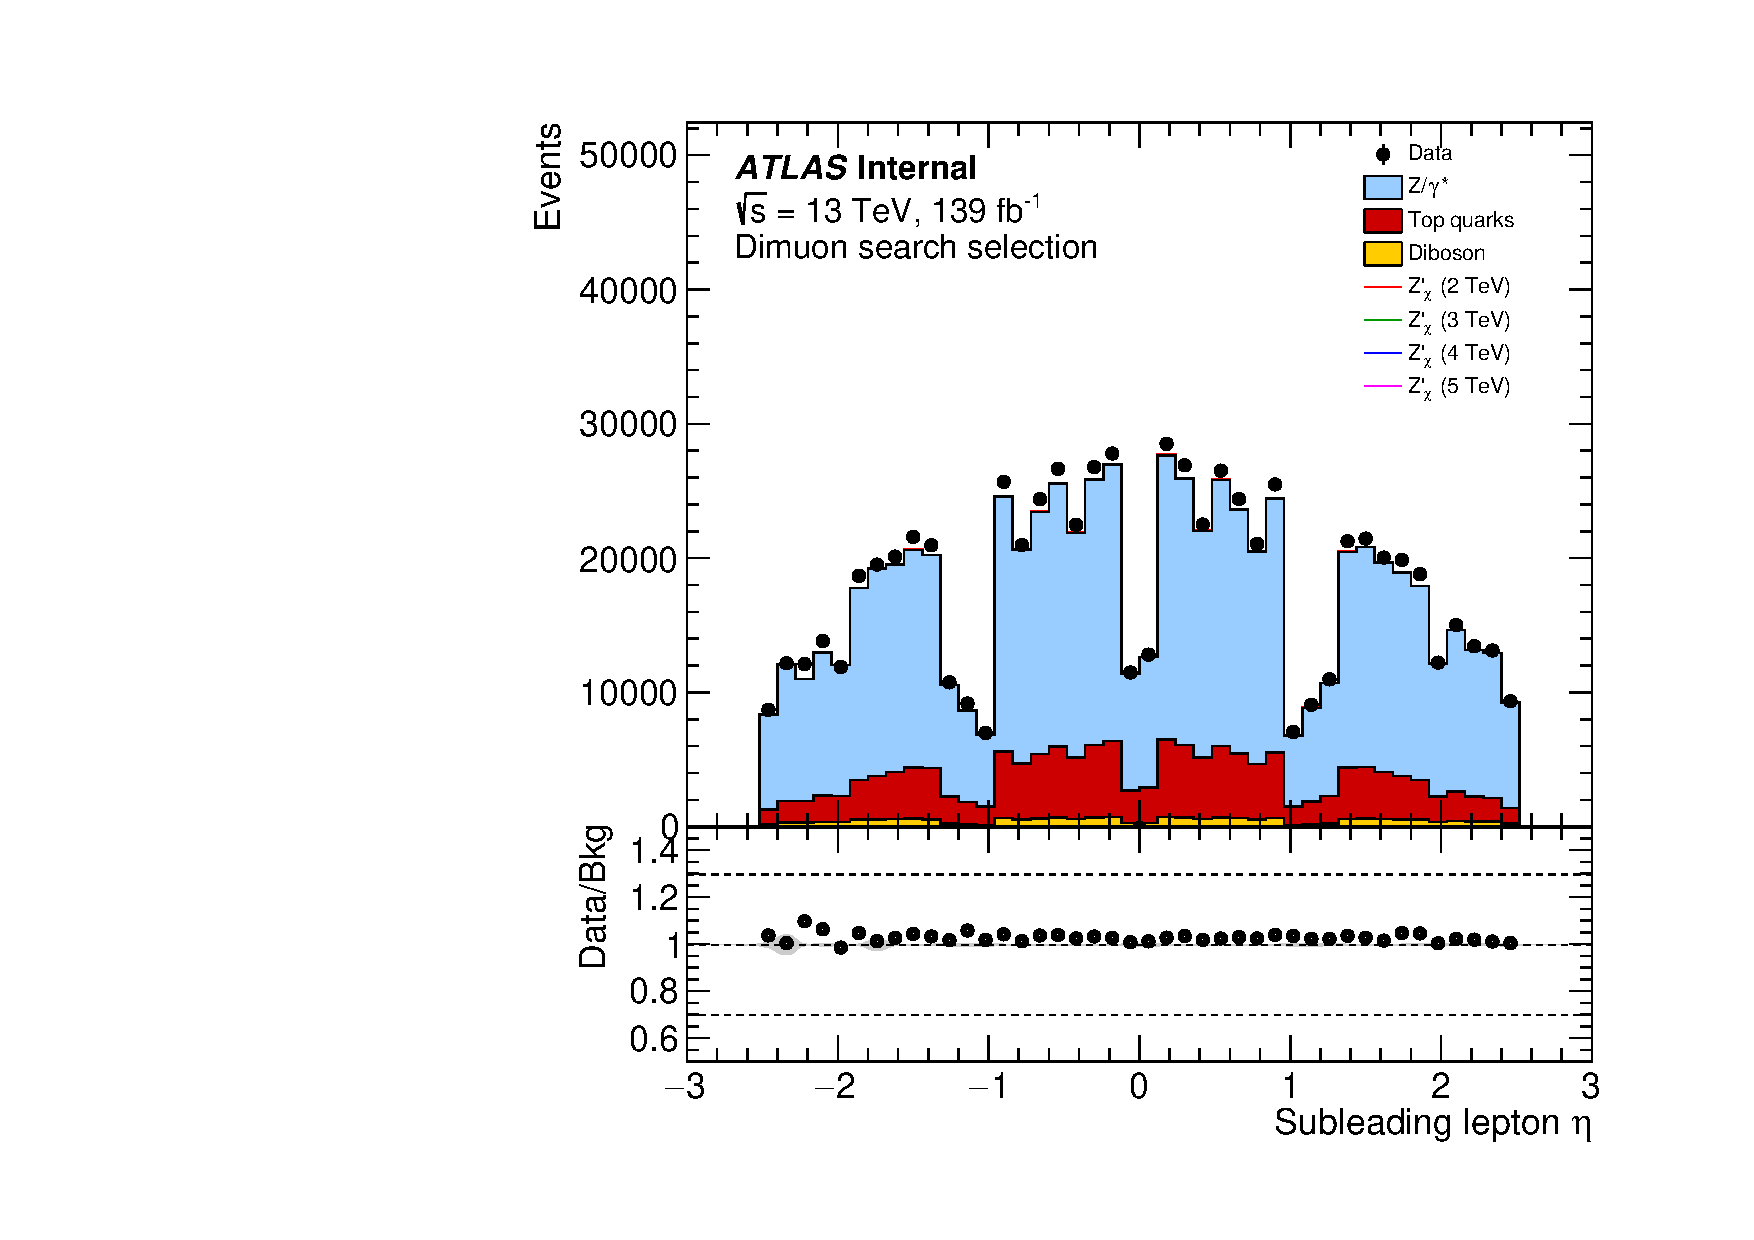
\includegraphics[width=1\textwidth]{figures/ci/dataMc/stacks_mc16e_2015-2018_uu_eta2.pdf}
    \subcaption{}
\end{minipage}\\
\begin{minipage}[b]{.45\linewidth}
    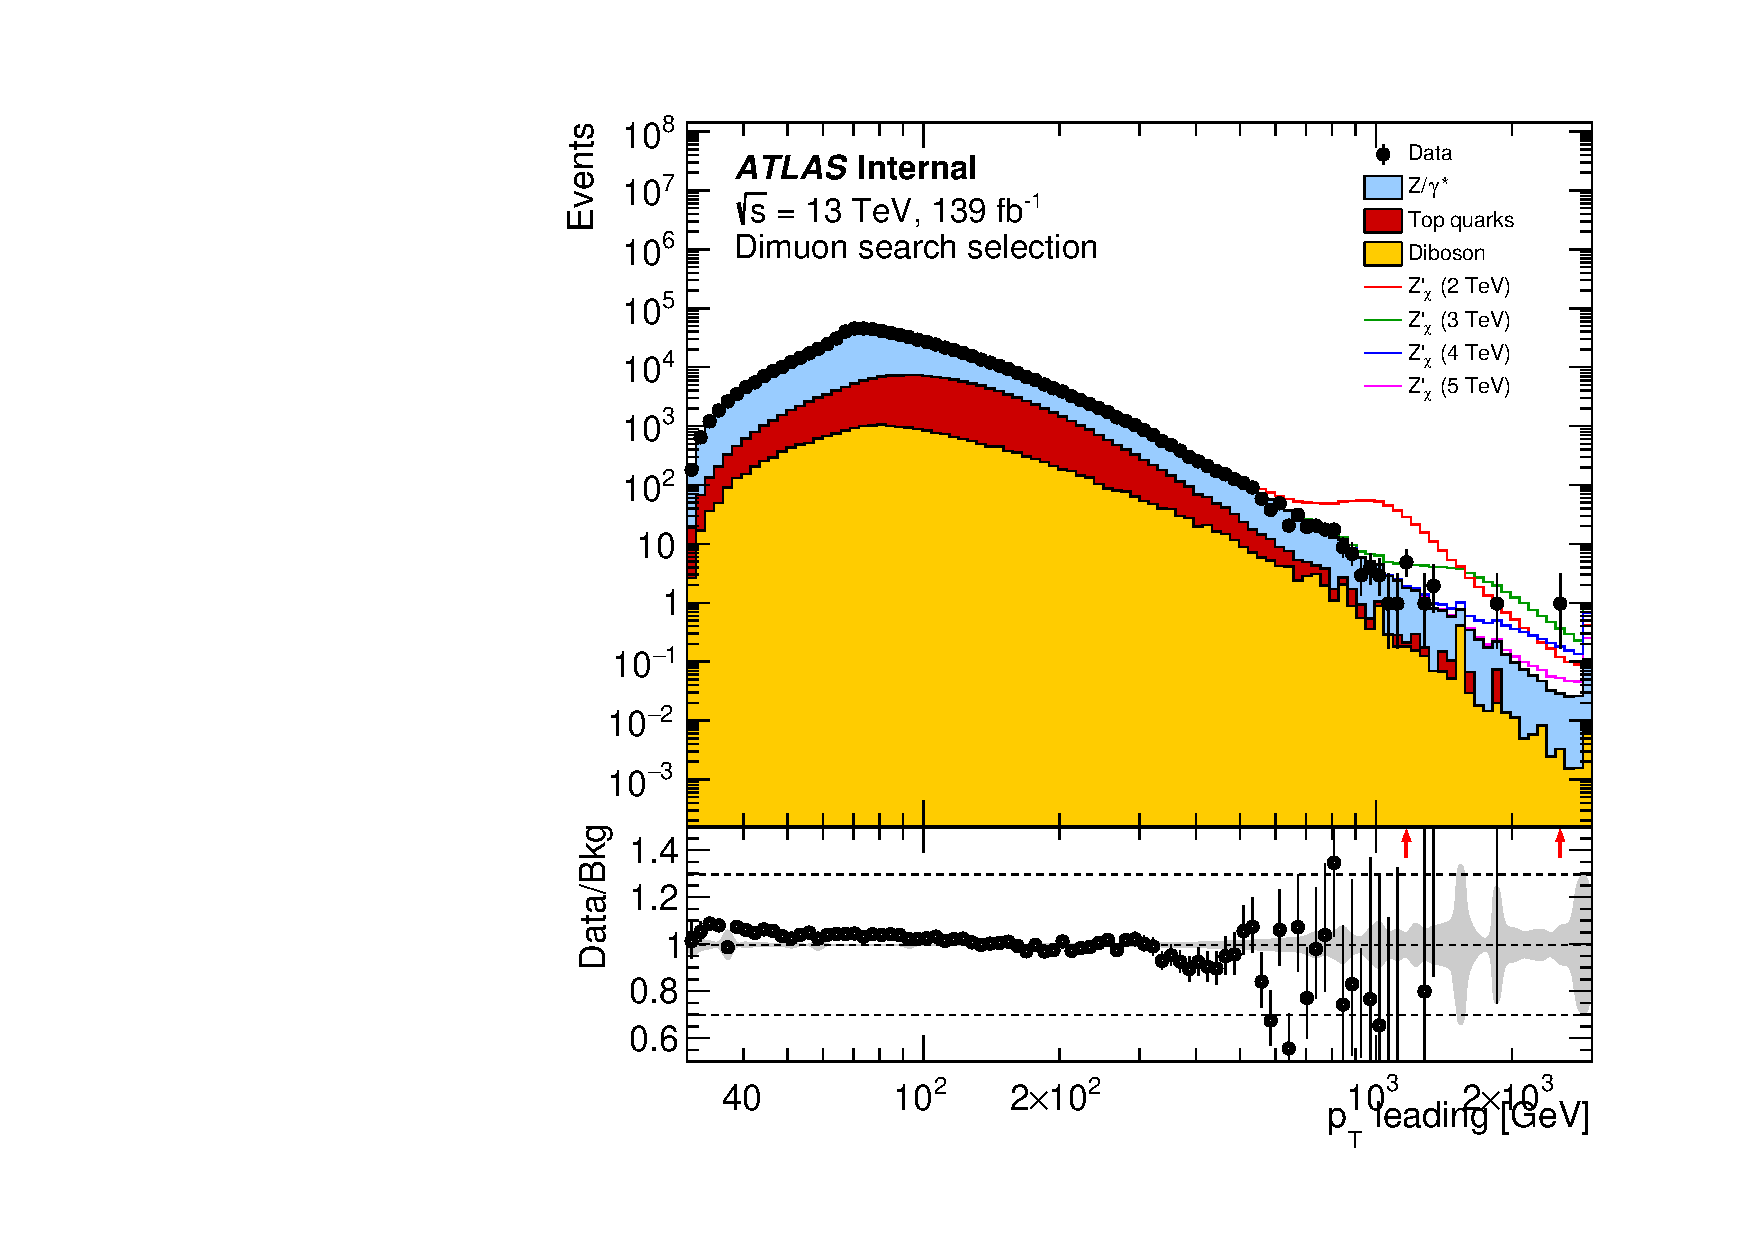
\includegraphics[width=1\textwidth]{figures/ci/dataMc/stacks_mc16e_2015-2018_uu_pt1_log100.pdf}
    \subcaption{}
\end{minipage}
\begin{minipage}[b]{.45\linewidth}
    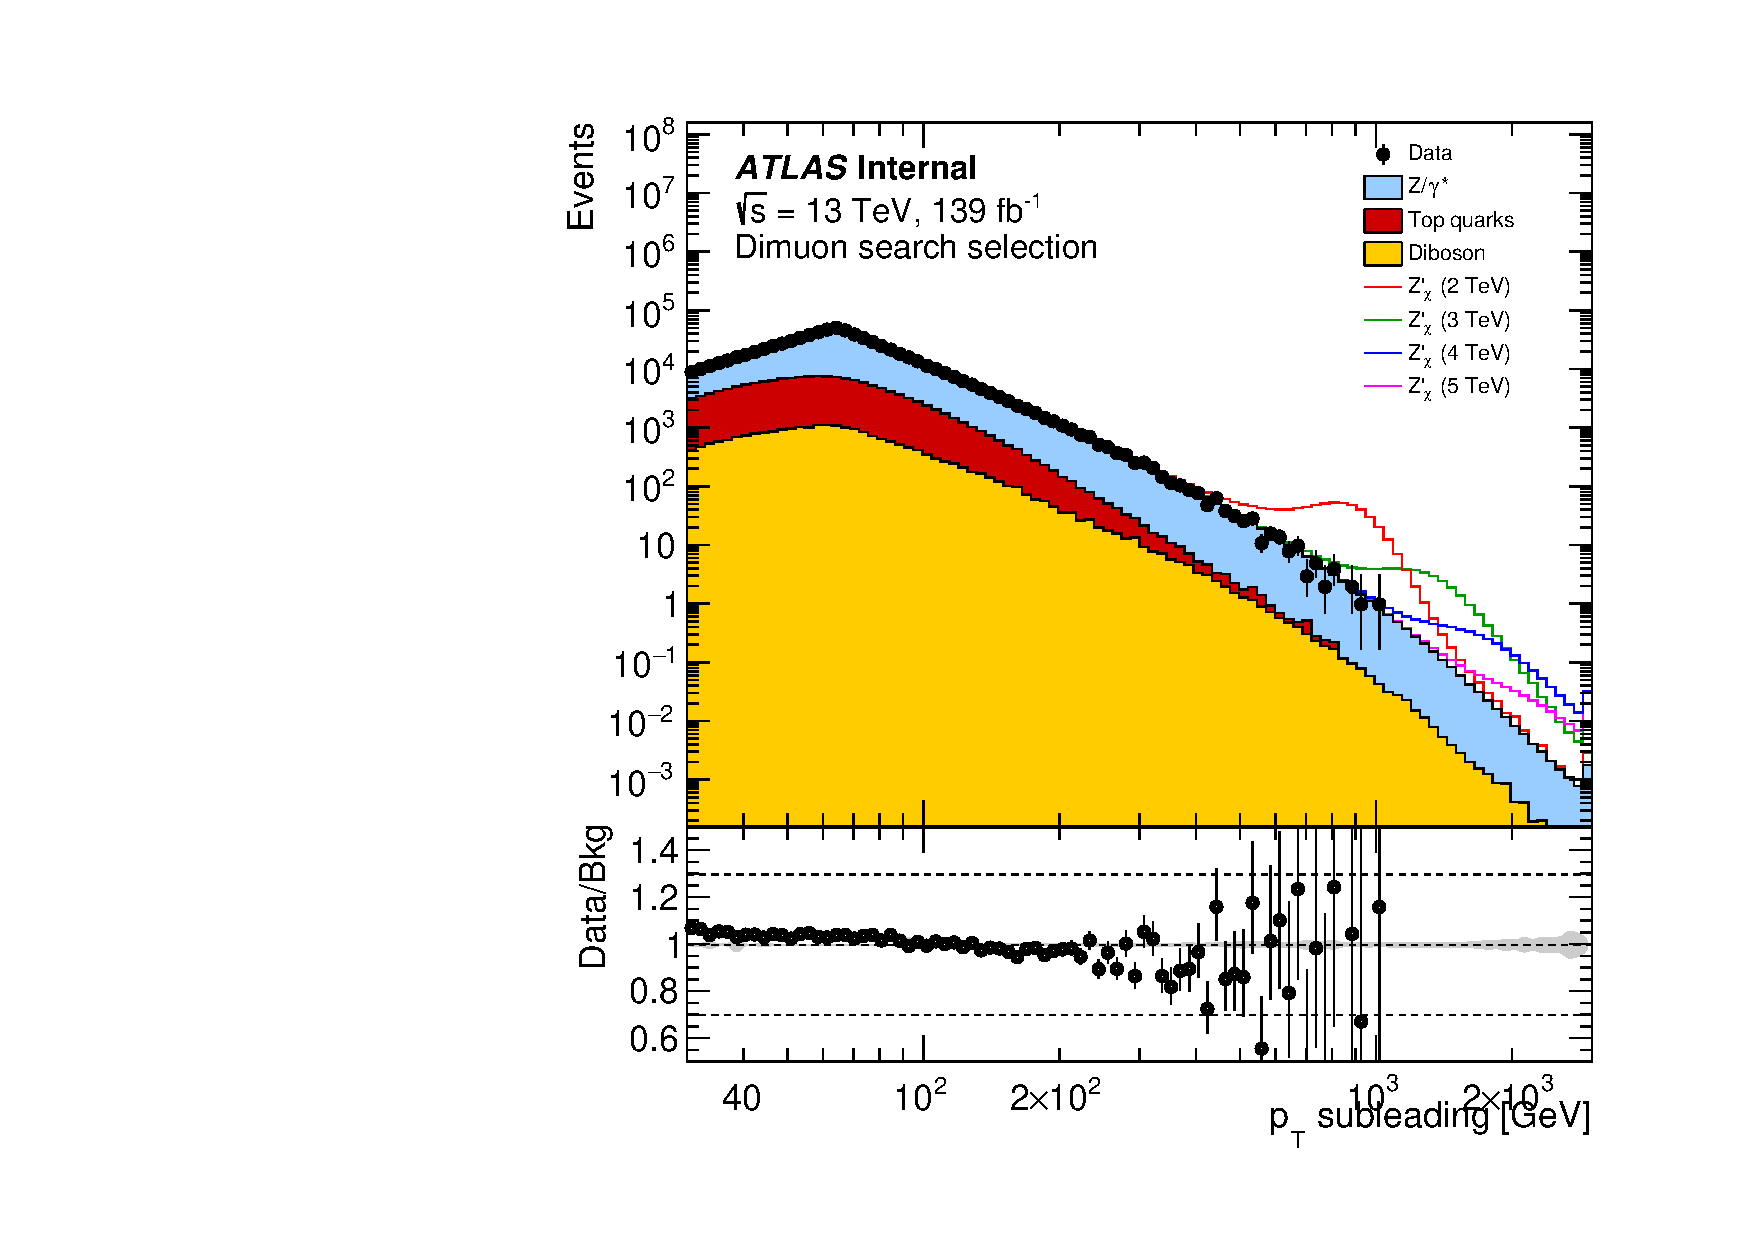
\includegraphics[width=1\textwidth]{figures/ci/dataMc/stacks_mc16e_2015-2018_uu_pt2_log100.pdf}
    \subcaption{}
\end{minipage}
\caption{Kinematic distributions in the $\mu\mu$ channel. (a) leading muon $\eta$, (b) subleading muon $\eta$, leading muon \pt, and subleading electron \pt.}
\label{fig:}
\end{figure}
\clearpage
}

\clearpage
